\documentclass[11pt,a4paper,openany]{scrbook}
% ============================================================
%  GLM PORTFOLIO -- SHARED PREAMBLE
%  Playful-but-structured design, ECRA phase system
% ============================================================

\usepackage[T1]{fontenc}
\usepackage[utf8]{inputenc}
\usepackage{charter}
\usepackage[scaled=0.92]{helvet}
\renewcommand{\familydefault}{\rmdefault}

\usepackage{amsmath,amssymb,amsthm}
\usepackage{xcolor}
\usepackage[most]{tcolorbox}
\usepackage{geometry}
\usepackage{titlesec}
\usepackage{fancyhdr}
\usepackage{enumitem}
\usepackage{graphicx}
\usepackage{tikz}
\usepackage{booktabs}
\usepackage{listings}
\usepackage[colorlinks=true,linkcolor=tealmain_,citecolor=tealmain_,urlcolor=amberacc_]{hyperref}
\usepackage[round]{natbib}
\usepackage{caption}

\geometry{a4paper, margin=2.6cm, headsep=1.1cm}

% avoid blank pages from \frontmatter/\mainmatter/\part forcing odd-page starts
\let\cleardoublepage\clearpage
\let\cleardoubleoddpage\clearpage
\let\cleardoubleevenpage\clearpage

% ---------- Colour palette ----------
% Core: teal (Cognition), amber (Reflection)
% Extended: slate-blue (Exploration), graphite (Application) -- tints/neutrals, not new loud hues
\definecolor{inkblack}{HTML}{1F2328}
\definecolor{tealmain}{HTML}{146C6E}
\definecolor{tealsoft}{HTML}{E3F2F1}
\definecolor{amberacc}{HTML}{D97C2B}
\definecolor{ambersoft}{HTML}{FBEBDA}
\definecolor{slateacc}{HTML}{3B5A76}
\definecolor{slatesoft}{HTML}{E9EFF4}
\definecolor{graphite}{HTML}{4B4F52}
\definecolor{graphitesoft}{HTML}{EDEDED}
\definecolor{greyline}{HTML}{9AA5A9}
\definecolor{mathsoft}{HTML}{F3F8F8}

% aliases so hyperref (loaded before some defs) can see the colours
\colorlet{tealmain_}{tealmain}
\colorlet{amberacc_}{amberacc}

\color{inkblack}

% ---------- Chapter / section styling ----------
\titleformat{\chapter}[display]
  {\normalfont\sffamily\bfseries}
  {\begin{tikzpicture}[remember picture,overlay]
     \fill[tealmain] (-0.45,-0.15) rectangle (-0.17,0.85);
   \end{tikzpicture}\color{greyline}\Large\MakeUppercase{\chaptertitlename} \thechapter}
  {6pt}
  {\color{tealmain}\Huge}
\titlespacing*{\chapter}{0pt}{10pt}{22pt}

\RedeclareSectionCommand[
  beforeskip=-10pt, afterskip=20pt,
  font=\normalfont\sffamily\bfseries\huge\color{tealmain}
]{part}
\renewcommand{\partformat}{\color{greyline}\sffamily\Large\MakeUppercase{\partname}~\thepart.\quad}

\titleformat{\section}
  {\normalfont\sffamily\bfseries\color{tealmain}\Large}{\thesection}{8pt}{}
\titleformat{\subsection}
  {\normalfont\sffamily\bfseries\color{amberacc}\large}{\thesubsection}{8pt}{}
\titleformat{\subsubsection}
  {\normalfont\sffamily\bfseries\color{amberacc}}{\thesubsubsection}{6pt}{}

\pagestyle{fancy}
\fancyhf{}
\renewcommand{\headrulewidth}{0.4pt}
\fancyhead[LE,RO]{\sffamily\small\thepage}
\fancyhead[RE]{\sffamily\small\nouppercase{\leftmark}}
\fancyhead[LO]{\sffamily\small\nouppercase{\rightmark}}

% ============================================================
%  ECRA PHASE SYSTEM
%  Each phase = a coloured banner heading + a matching box style
% ============================================================

% ---- generic phase-banner heading ----
\newcommand{\phaseheading}[2]{%
  \vspace{14pt}
  \noindent\colorbox{#1}{\parbox{\dimexpr\linewidth-12pt}{\vspace{3pt}\sffamily\bfseries\color{white}\large #2\vspace{3pt}}}%
  \vspace{8pt}\par
}

% ---- EXPLORATION: slate-blue, "browser frame" screenshot box ----
\newcommand{\Exploration}{\phaseheading{slateacc}{Exploration}}

\newenvironment{screenshot}[1][]{%
  \begin{center}
  \begin{tcolorbox}[
    colback=white, colframe=slateacc, boxrule=0.6pt, arc=1pt,
    width=0.92\linewidth,
    top=2pt,bottom=2pt,left=2pt,right=2pt,
    before skip=8pt, after skip=4pt
  ]
  \ifx\\#1\\\else{\sffamily\footnotesize\color{slateacc} #1}\\[2pt]\fi
}{%
  \end{tcolorbox}
  \end{center}
}

% informal exploration-phase source note (not a formal \cite)
\newcommand{\explorationsource}[1]{{\sffamily\footnotesize\color{slateacc} Source: #1}}

% ---- COGNITION: teal, definitions + theorems + formal citation ----
\newcommand{\Cognition}{\phaseheading{tealmain}{Cognition}}

\newtcolorbox{defbox}[1][]{
  colback=tealsoft, colframe=tealmain, boxrule=0.6pt, arc=2pt,
  fonttitle=\sffamily\bfseries, title={Definition#1},
  left=8pt,right=8pt,top=5pt,bottom=5pt
}
\newtheorem{theorem}{Theorem}[chapter]
\newtheorem{lemma}[theorem]{Lemma}
\newtheorem{proposition}[theorem]{Proposition}
\renewcommand{\qedsymbol}{$\blacksquare$}

% glossary-style term heading (for Chapter 3's Language of GLMs)
\newcommand{\term}[1]{\vspace{4pt}\subsubsection*{\sffamily\bfseries\color{tealmain} #1}}

% unnumbered chapter heading (Part IV evaluation topics), same visual family, no "Chapter N" tab
\newcommand{\uchapter}[1]{%
  \clearpage
  \phantomsection
  \vspace*{10pt}
  {\sffamily\bfseries\color{tealmain}\huge #1\par}
  \vspace{18pt}
  \addcontentsline{toc}{chapter}{#1}
  \markboth{#1}{#1}
}

% ---- REFLECTION: amber, question/exercise boxes ----
\newcommand{\Reflection}{\phaseheading{amberacc}{Reflection}}

\newtcolorbox{questionbox}[1][]{
  colback=ambersoft, colframe=amberacc, boxrule=0.6pt, arc=2pt,
  fonttitle=\sffamily\bfseries, title={Question#1},
  left=8pt,right=8pt,top=5pt,bottom=5pt
}

% ---- APPLICATION: graphite/neutral, code ----
\newcommand{\Application}{\phaseheading{graphite}{Application}}

\lstdefinestyle{rcode}{
  backgroundcolor=\color{graphitesoft},
  basicstyle=\ttfamily\footnotesize\color{inkblack},
  keywordstyle=\color{tealmain}\bfseries,
  commentstyle=\color{greyline}\itshape,
  numberstyle=\tiny\color{greyline},
  stringstyle=\color{amberacc},
  numbers=left,
  numbersep=8pt,
  frame=single,
  rulecolor=\color{greyline},
  framerule=0.4pt,
  breaklines=true,
  showstringspaces=false,
  xleftmargin=10pt,
  framexleftmargin=6pt
}
\lstset{style=rcode}

% "to be completed" placeholder, styled quietly so it doesn't compete visually
\newcommand{\tbc}{{\sffamily\itshape\color{greyline} To be completed.}\par\vspace{6pt}}

% ============================================================
%  MATH HIGHLIGHT DESIGN
%  Every standalone display equation gets its own subtle
%  highlighted band, distinguishing math from prose at a glance.
% ============================================================
\usepackage[framemethod=TikZ]{mdframed}
\mdfdefinestyle{mathstyle}{
  backgroundcolor=mathsoft,
  linecolor=tealmain,
  linewidth=0pt,
  leftline=true,
  topline=false,
  bottomline=false,
  rightline=false,
  linewidth=2.5pt,
  innerleftmargin=12pt,
  innerrightmargin=8pt,
  innertopmargin=6pt,
  innerbottommargin=6pt,
  skipabove=8pt,
  skipbelow=8pt
}
\newmdenv[style=mathstyle]{mathbox}


\begin{document}

% ================= TITLE PAGE =================
\begin{titlepage}
\begin{tikzpicture}[remember picture,overlay]
  \fill[tealmain] (current page.north west) rectangle ([yshift=-3.2cm]current page.north east);
  \fill[amberacc] (current page.south west) rectangle ([yshift=0.55cm]current page.south east);
\end{tikzpicture}
\vspace*{4.6cm}
\begin{flushleft}
\hspace{0.2cm}
\begin{minipage}{0.9\textwidth}
{\sffamily\bfseries\huge\color{tealmain} Generalised Linear Models}\\[6pt]
{\sffamily\Large\color{amberacc} A Portfolio}\\[26pt]
{\sffamily\large\color{inkblack} An Exploration--Cognition--Reflection--Application journey through GLM theory}\\[60pt]
{\sffamily\color{greyline} Dominion Oamen}\\
{\sffamily\small\color{greyline} University of the Free State}
\end{minipage}
\end{flushleft}
\end{titlepage}

\frontmatter
\tableofcontents

\chapter*{Foreword}
\addcontentsline{toc}{chapter}{Foreword}

This portfolio began as an attempt to capture my journey from absolute uncertainty to a solid grasp of Generalised Linear Models. My aim is to document not just the concepts, but the problems I encountered, the questions I asked, and how I went about answering them.

Traditional note-taking usually amounts to writing down vague, cognitively disconnected concepts that teach the how without ever establishing the why. This portfolio takes the opposite approach: it moves slowly through the why before arriving at the how.

To ground these concepts in something real, one dataset runs throughout this entire portfolio: nitrogen fertilizer applied against potato yield. Working with the same data across every chapter surfaces questions that never show up when the math and terminology are understood only in the abstract.

I have not approached this portfolio like a textbook, even though it covers essentially all the mathematics needed for a first course in GLMs. Instead, the structure follows the shape of the problem itself: try something, watch it fail, ask why it failed, then build the solution that addresses that specific failure. Each chapter is a pathway from problem to solution rather than a definition waiting to be memorised.

By the end of this portfolio, a reader should understand why we speak about generalised linear models at all, the mathematics underlying them, how to fit a GLM, and how to interpret its results. As an added bonus, I also cover dimensionality reduction using Permutation Variable Importance in Python via DALEX, since knowing which variables actually matter, and which can safely be dropped, is a skill that bridges data engineering and data analysis. Python handles that variable selection step; R handles the GLM fitting itself, since it has strong built-in support for it.

Partway through this portfolio I settled on a study technique I call \textbf{ECRA}: \textbf{E}xploration, \textbf{C}ognition, \textbf{R}eflection, \textbf{A}pplication. Each chapter, where the ECRA structure applies, moves through these four phases in order: Exploration is the informal, beginner's first contact with a concept (a video, a search, an intuition); Cognition is where things get formal, with definitions and derivations; Reflection is where I step back and interrogate what actually landed and what didn't; and Application is where the concept gets used, tested, or simulated. Some phases are still blank while I work through the material; those are marked accordingly.

Without further ado, let's start this journey together.

\mainmatter

% ================= PART I =================
\part{Introduction to GLMs}

\chapter{OLS}

\Exploration

At this point in the chapter I approach OLS as a total beginner trying to explore the concept of Ordinary Least Squares. To start, the best way to approach any exploration of new concepts is to research using YouTube University, so I searched ``OLS'' on YouTube and got this.

\begin{screenshot}
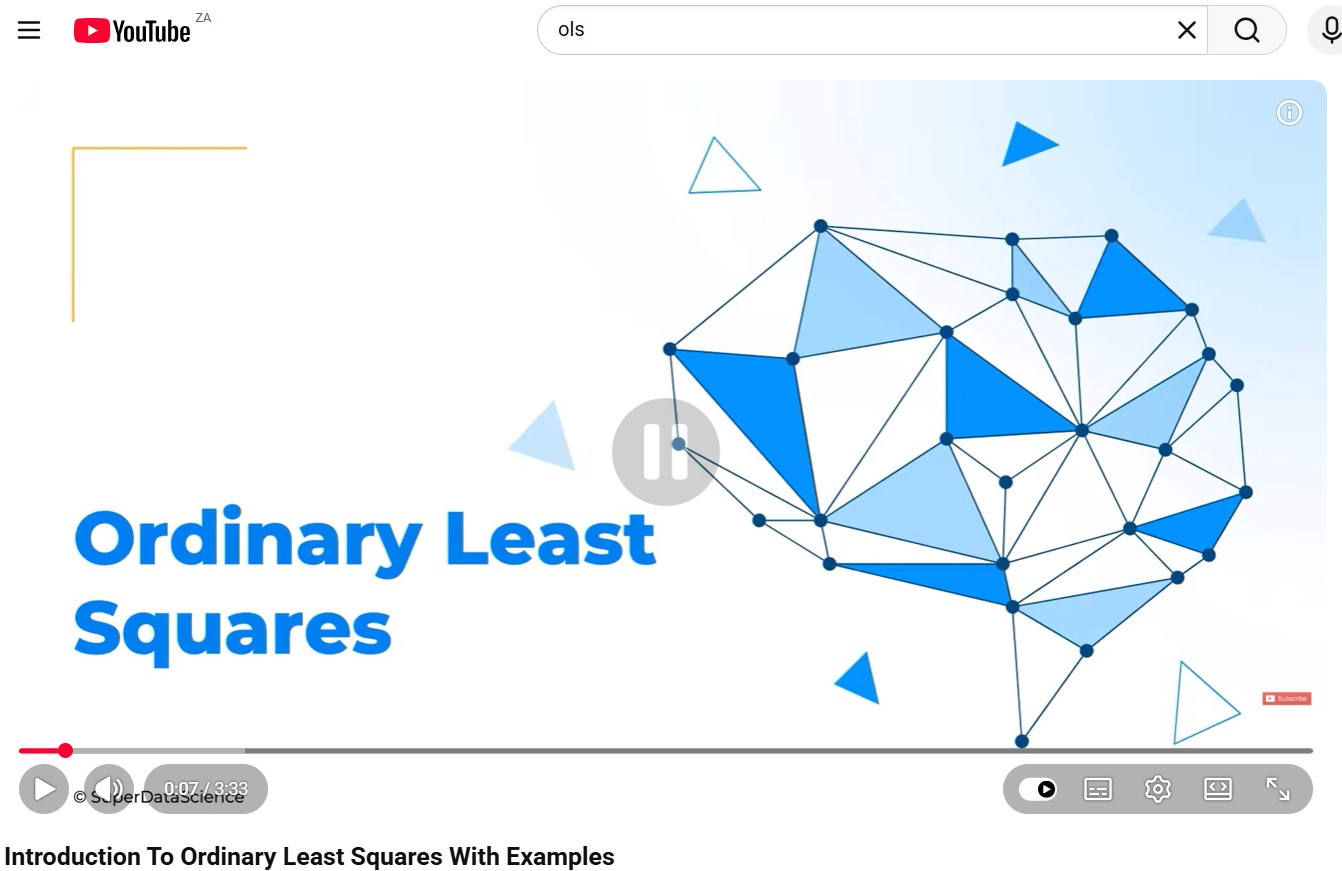
\includegraphics[width=\linewidth]{assets/exploration-youtube-ols.png}
\end{screenshot}
\captionof{figure}{OLS video from YouTube \citep{sds2023}.}
\explorationsource{Super Data Science (2023), \textit{Introduction to Ordinary Least Squares with Examples}, YouTube.}

\vspace{6pt}
So what is ``Ordinary Least Squares''?

This image is a practical example of OLS (linear regression) showing the line of best fit, model accuracy, and sum of squares (minimised).

\begin{screenshot}
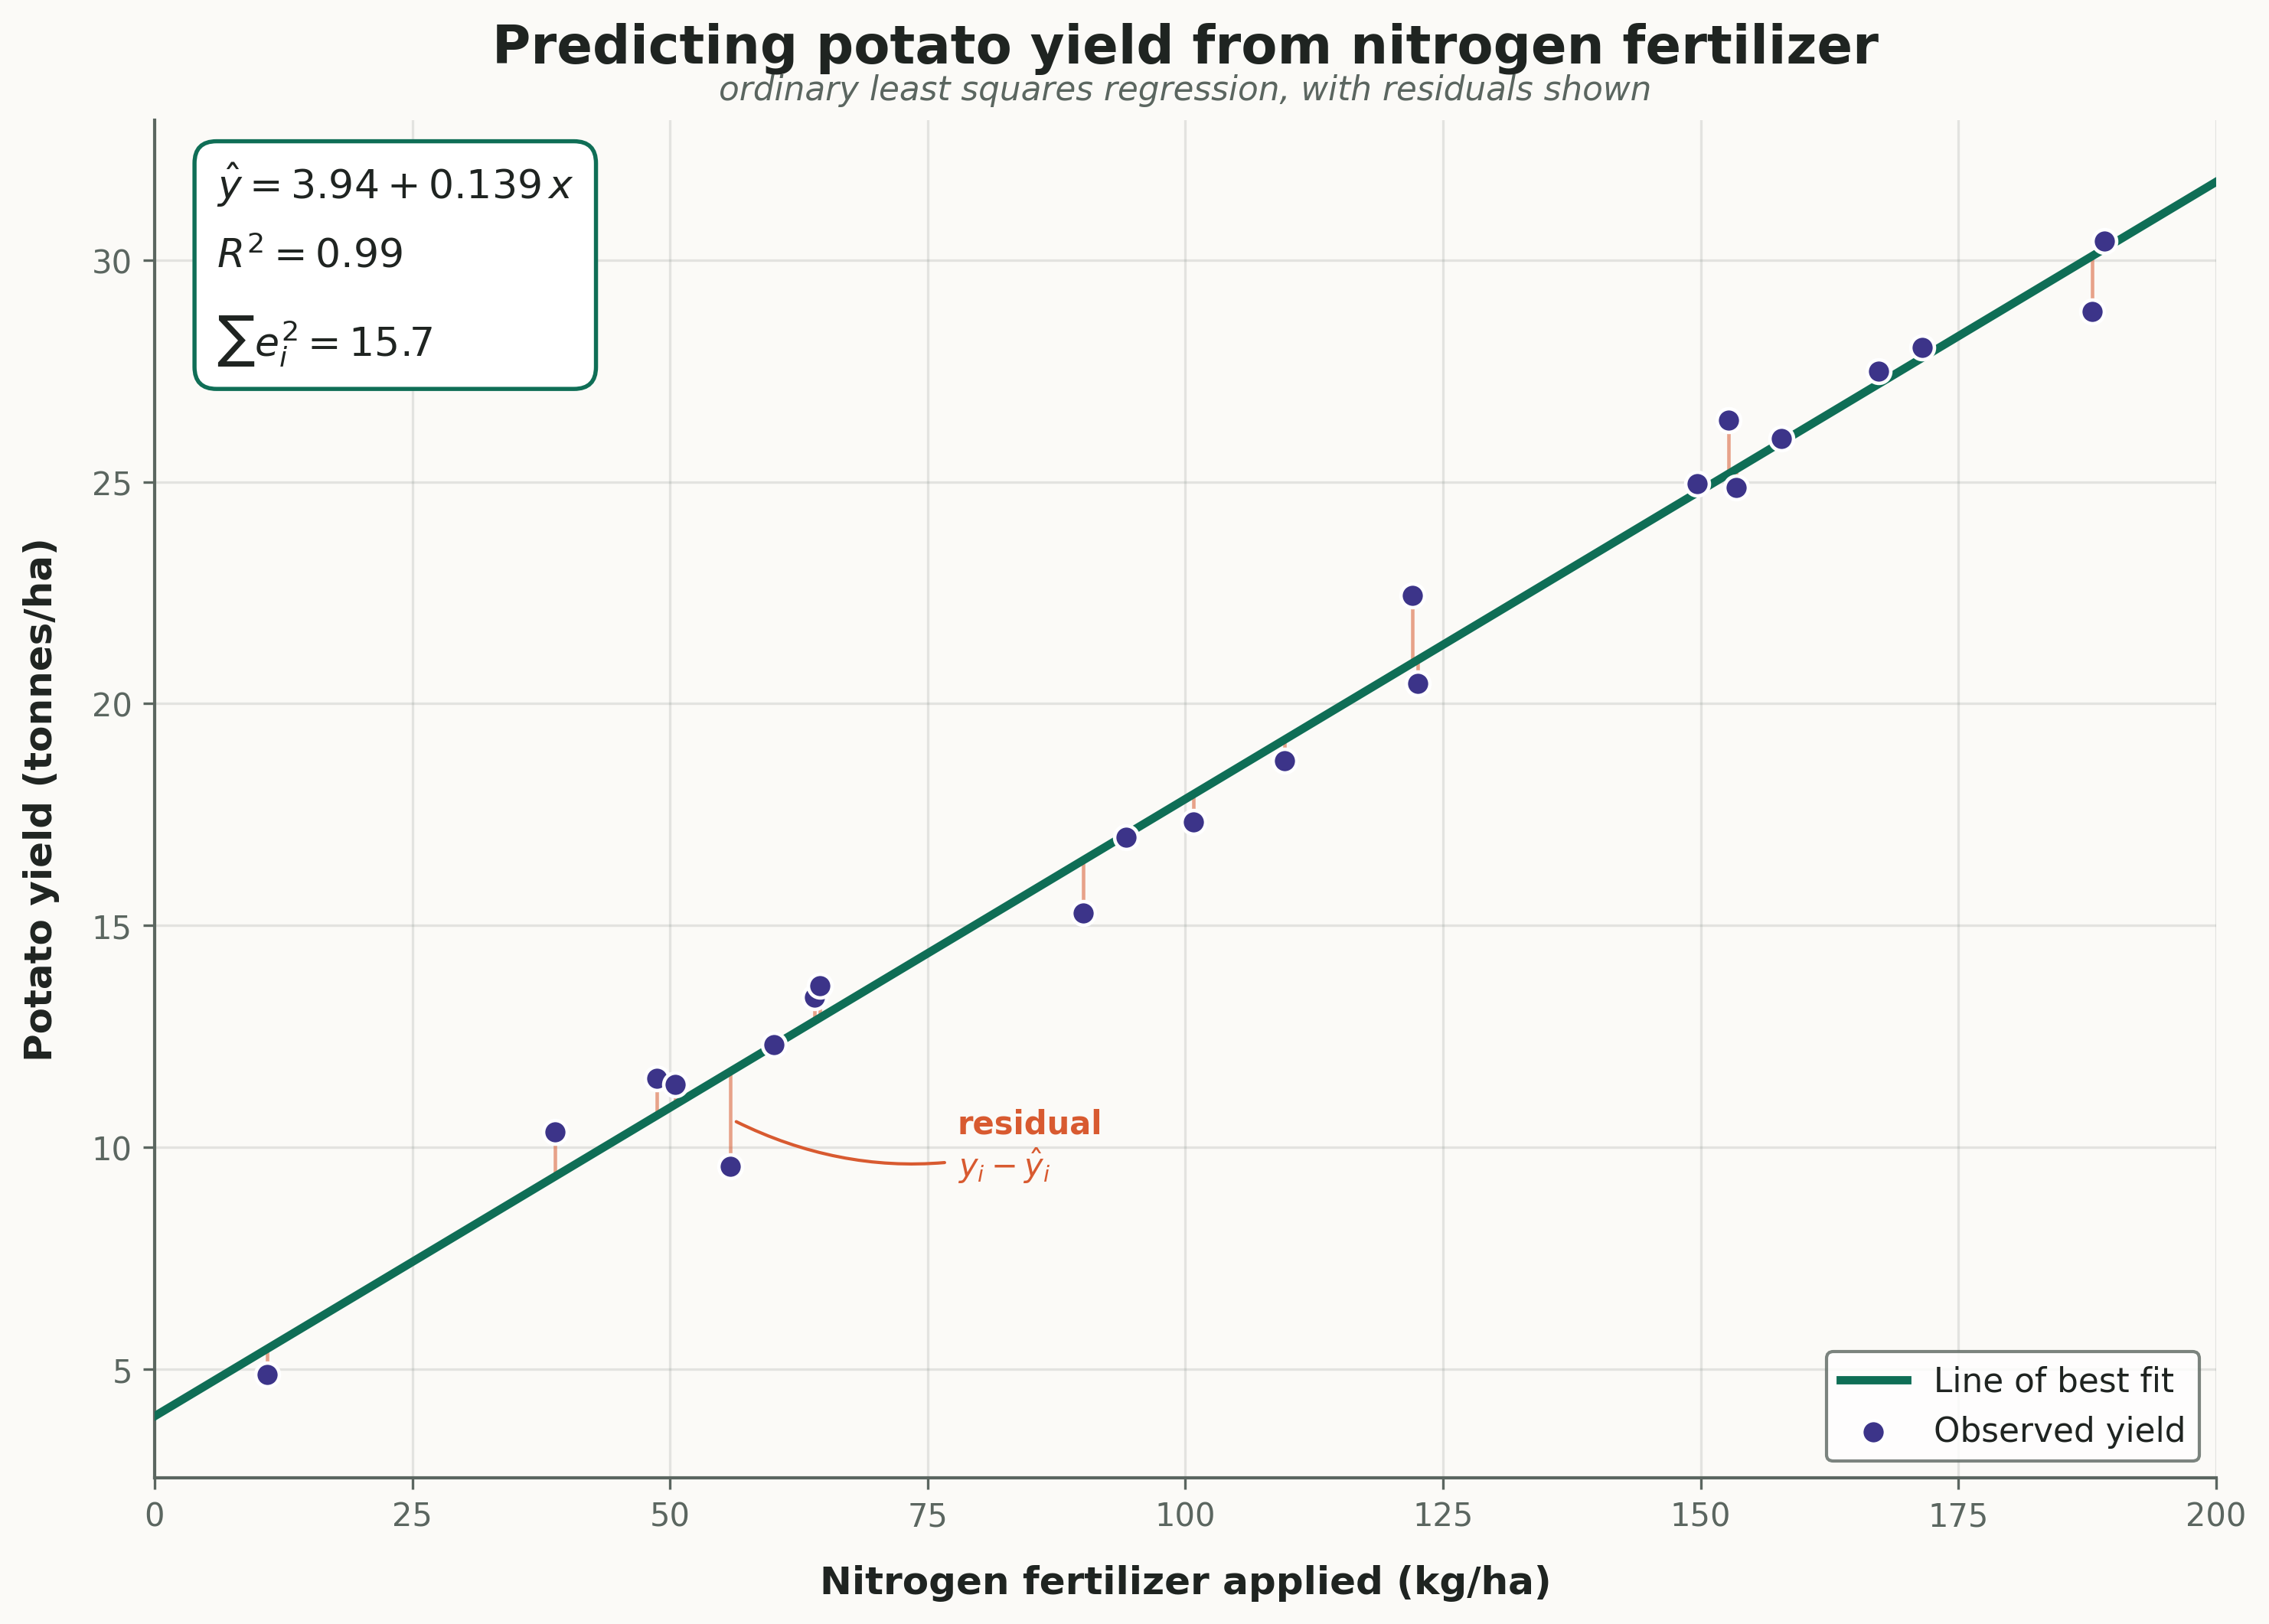
\includegraphics[width=0.85\linewidth]{assets/exploration-ols-example.png}
\end{screenshot}
\captionof{figure}{A practical example of OLS (linear regression): the line of best fit, model accuracy, and the (minimised) sum of squares.}

We move further to the Cognition phase, where things get more formal and definitions and some fun maths appear.

\Cognition

\subsection*{Linear Regression}
A model used in statistics to assess the connection between a scalar response (dependent variable) and one or more explanatory factors (independent variables or regressors) is called linear regression.
\begin{mathbox}
\[
y_i = \beta_0 + \beta_1 x_i + \epsilon_i
\]
\end{mathbox}

\subsection*{Simple Linear Regression}
A linear regression with just one explanatory variable. It is a clear system with no confounding, where cause is most likely linked directly to effect.

\subsection*{Multiple Linear Regression}
A linear regression with two or more explanatory variables. It is more interesting and more prone to confounding, since cause doesn't always mean effect; it could be a combination of causes, or a cause could appear prominent only because of another variable.

To see why the exponential family occupies such a central place in GLM theory, it helps to start with the simple linear model.

\subsection*{The Linear Model as a Starting Point}
The simple linear model is written
\begin{mathbox}
\[
Y_i = \beta_0 + \beta_1 x_i + \epsilon_i
\]
\end{mathbox}
where $\epsilon_i$ is an error term assumed to be normally distributed with mean 0 and constant variance $\sigma^2$, that is $\epsilon_i \sim N(0,\sigma^2)$. Because $Y_i$ is a constant $(\beta_0+\beta_1 x_i)$ plus a normally distributed random variable, $Y_i$ itself is normally distributed:
\begin{mathbox}
\[
Y_i \sim N(\mu_i,\sigma^2), \qquad \mu_i = \beta_0 + \beta_1 x_i
\]
\end{mathbox}

In other words, the linear combination of the explanatory variable and its coefficient does not directly define $Y_i$, it defines where the mean of $Y_i$ sits. The error term provides the randomness and its distributional form, while the linear predictor $\beta_0+\beta_1 x_i$ simply drags that mean to where the covariate $x_i$ indicates it should be. This separation, a distributional assumption on one side and a linear predictor governing the mean on the other, is precisely what GLMs later generalise.

\subsection*{Extending to Multiple Explanatory Variables and Vector Responses}
The same logic extends naturally once there is more than one explanatory variable. Instead of a single $x_i$, we have a row of covariates for each observation, and the mean becomes
\begin{mathbox}
\[
\mu_i = \beta_0 + \beta_1 x_{i1} + \beta_2 x_{i2} + \cdots + \beta_p x_{ip} = x_i^\top \beta
\]
\end{mathbox}
with $Y_i \sim N(\mu_i,\sigma^2)$ still holding, only now $\mu_i$ is a linear combination of several predictors rather than one. Written for the whole sample at once, this is $Y = X\beta + \epsilon$, with $X$ the design matrix and $\beta$ the vector of coefficients.

\subsection*{Where the Linear Model Falls Short}
The assumptions underpinning the linear model, constant variance, a normally distributed response, and a mean that varies linearly with the predictors, do not hold for a great deal of real data. Counts of events, binary outcomes (success/failure), and proportions are common, none of which are well described by a normal distribution with constant variance. A count cannot be negative, and its variance tends to grow with its mean; a binary outcome only takes two values; a proportion is bounded between 0 and 1.

There is also the question of the relationship between the response mean and the linear predictor. In the classical linear model that relationship is direct: $\mu_i$ literally equals the linear combination of covariates. But for many response types above, a straight linear relationship on the original scale does not make sense; for a binary outcome, what varies linearly with the covariates is more naturally the log-odds of success (the logit) rather than the probability itself.

Historically, fitting anything outside the normal linear model was difficult because closed-form estimators generally do not exist once the response distribution departs from normality or the mean is connected to the predictors through a nonlinear transformation. Iterative fitting procedures, developed to extend maximum likelihood estimation into settings without closed-form solutions, changed this: estimation still proceeds via an iteratively reweighted least-squares computation, echoing the linear model even as the distributional assumptions underlying it change entirely.

\subsection*{Deriving the Normal Equations by Hand}
For simple linear regression, we are fitting $\hat y_i = \beta_0+\beta_1 x_i$, with residual $e_i = y_i - \hat y_i$. Residuals are not summed directly, since positive and negative errors would cancel; instead the sum of squared residuals is minimised,
\begin{mathbox}
\[
S(\beta_0,\beta_1) = \sum_{i=1}^n \left(y_i - \beta_0 - \beta_1 x_i\right)^2
\]
\end{mathbox}

\begin{theorem}[Normal Equations]
Differentiating $S(\beta_0,\beta_1)$ with respect to each parameter and setting both to zero gives the normal equations \citep{dobson2018,casella2002}:
\begin{mathbox}
\[
\frac{\partial S}{\partial \beta_0} = -2\sum_{i=1}^n \left(y_i-\beta_0-\beta_1 x_i\right) = 0, \qquad
\frac{\partial S}{\partial \beta_1} = -2\sum_{i=1}^n x_i\left(y_i-\beta_0-\beta_1 x_i\right) = 0
\]
\end{mathbox}
Expanding the first and solving for $\beta_0$ gives $\beta_0 = \bar y - \beta_1\bar x$, which also shows the fitted line always passes through $(\bar x,\bar y)$. Substituting this into the second equation and simplifying gives the slope,
\begin{mathbox}
\[
\beta_1 = \frac{\sum_{i=1}^n (x_i-\bar x)(y_i-\bar y)}{\sum_{i=1}^n (x_i-\bar x)^2}
\]
\end{mathbox}
the covariance of $x$ and $y$ divided by the variance of $x$. Because $S(\beta_0,\beta_1)$ is a sum of squares, it is convex, so the second-order conditions are automatically satisfied and this stationary point is guaranteed to be a minimum.
\end{theorem}

\subsection*{Matrix Form of OLS}
The scalar derivation generalises directly to any number of predictors. Stacking the data gives $Y = X\beta+\epsilon$, with fitted values $\hat Y = X\beta$ and residual vector $e=Y-X\beta$. The sum of squared residuals is
\begin{mathbox}
\[
S(\beta) = e^\top e = (Y-X\beta)^\top(Y-X\beta) = Y^\top Y - 2\beta^\top X^\top Y + \beta^\top X^\top X \beta
\]
\end{mathbox}
Differentiating with respect to $\beta$ using the standard identities $\partial(\beta^\top X^\top Y)/\partial\beta = X^\top Y$ and $\partial(\beta^\top X^\top X\beta)/\partial\beta = 2X^\top X\beta$ \citep{casella2002}, and setting the result to zero, gives the normal equations in matrix form, $X^\top X\beta = X^\top Y$. Provided $X^\top X$ is invertible,
\begin{mathbox}
\[
\hat\beta = (X^\top X)^{-1}X^\top Y
\]
\end{mathbox}
which is exactly the closed-form estimator introduced as a term in Chapter 3, now derived rather than quoted. The Hessian $2X^\top X$ is positive semi-definite by construction, confirming this stationary point is a minimum \citep{dobson2018}. Rearranging $X^\top X\hat\beta = X^\top Y$ also gives $X^\top(Y-X\hat\beta)=0$, i.e.\ $X^\top e = 0$: the residual vector is orthogonal to every column of $X$, the orthogonality condition referenced under the Transposed Matrix term.

\Reflection

Looking back on the process of learning Ordinary Least Squares, I can say with confidence that I now understand both the intuition behind it and the mathematics underpinning it. Two questions arose along the way and were already answered, in passing, during the Cognition phase. Naming a question clearly is often what turns a passively absorbed derivation into a properly internalised one.

\begin{questionbox}[: Why do we need models at all?]
A model is a representation of a real-world process, constructed so that inferences can be made about the future behaviour of that process without repeating the underlying experiment every time. An experiment cannot be run on a future outcome, since that outcome does not yet exist empirically; data collection is also costly, so it would be far from optimal to repeat an experiment in full each time a new inference is required. The most intuitive model of all is a straight line, the line of best fit, from which it becomes possible both to predict future outcomes and to quantify how wrong those predictions are likely to be.
\end{questionbox}

\begin{questionbox}[: Why are the residuals squared before being summed?]
Each residual measures how wrong a single prediction is, and each residual carries a sign. Summing the residuals directly would allow positive and negative errors to cancel, leaving only the net direction in which predictions err rather than their overall magnitude. Squaring removes the sign while preserving, and emphasising, the size of the deviation. The resulting sum of squared errors is the quantity Ordinary Least Squares minimises.
\end{questionbox}

\Application

To put the theory into practice, a dataset was simulated in R to echo the exploration-phase example: nitrogen fertilizer applied (kg/ha) as the predictor, and potato yield (tonnes/ha) as the response, generated from the true relationship $y = 3.94 + 0.139x + \epsilon$ with $\epsilon \sim N(0, 0.55^2)$, so that the simulated data would recover a fit close to the original figure while remaining a fresh, reproducible dataset in its own right.

\begin{lstlisting}[language=R, caption={Simulating the dataset and fitting it with lm()}]
set.seed(2026)
n <- 25

# Nitrogen fertilizer applied, kg/ha
nitrogen <- round(runif(n, min = 10, max = 190), 1)

# True relationship (matches the exploration-phase figure)
beta0_true <- 3.94
beta1_true <- 0.139
sigma <- 0.55

yield <- beta0_true + beta1_true * nitrogen + rnorm(n, mean = 0, sd = sigma)
yield <- round(pmax(yield, 0), 2)

potato_yield_data <- data.frame(
  nitrogen_kg_ha = nitrogen,
  yield_tonnes_ha = yield
)

fit <- lm(yield_tonnes_ha ~ nitrogen_kg_ha, data = potato_yield_data)
summary(fit)
\end{lstlisting}

\begin{lstlisting}[language=R, caption={Output of summary(fit)}]
Coefficients:
              Estimate Std. Error t value Pr(>|t|)
(Intercept)   3.864663   0.203246   19.02  1.45e-15 ***
nitrogen_kg_ha 0.137992  0.002323   59.40  < 2e-16 ***

Residual standard error: 0.5296 on 23 degrees of freedom
Multiple R-squared: 0.9935, Adjusted R-squared: 0.9932
F-statistic: 3529 on 1 and 23 DF, p-value: < 2.2e-16
\end{lstlisting}

\begin{screenshot}
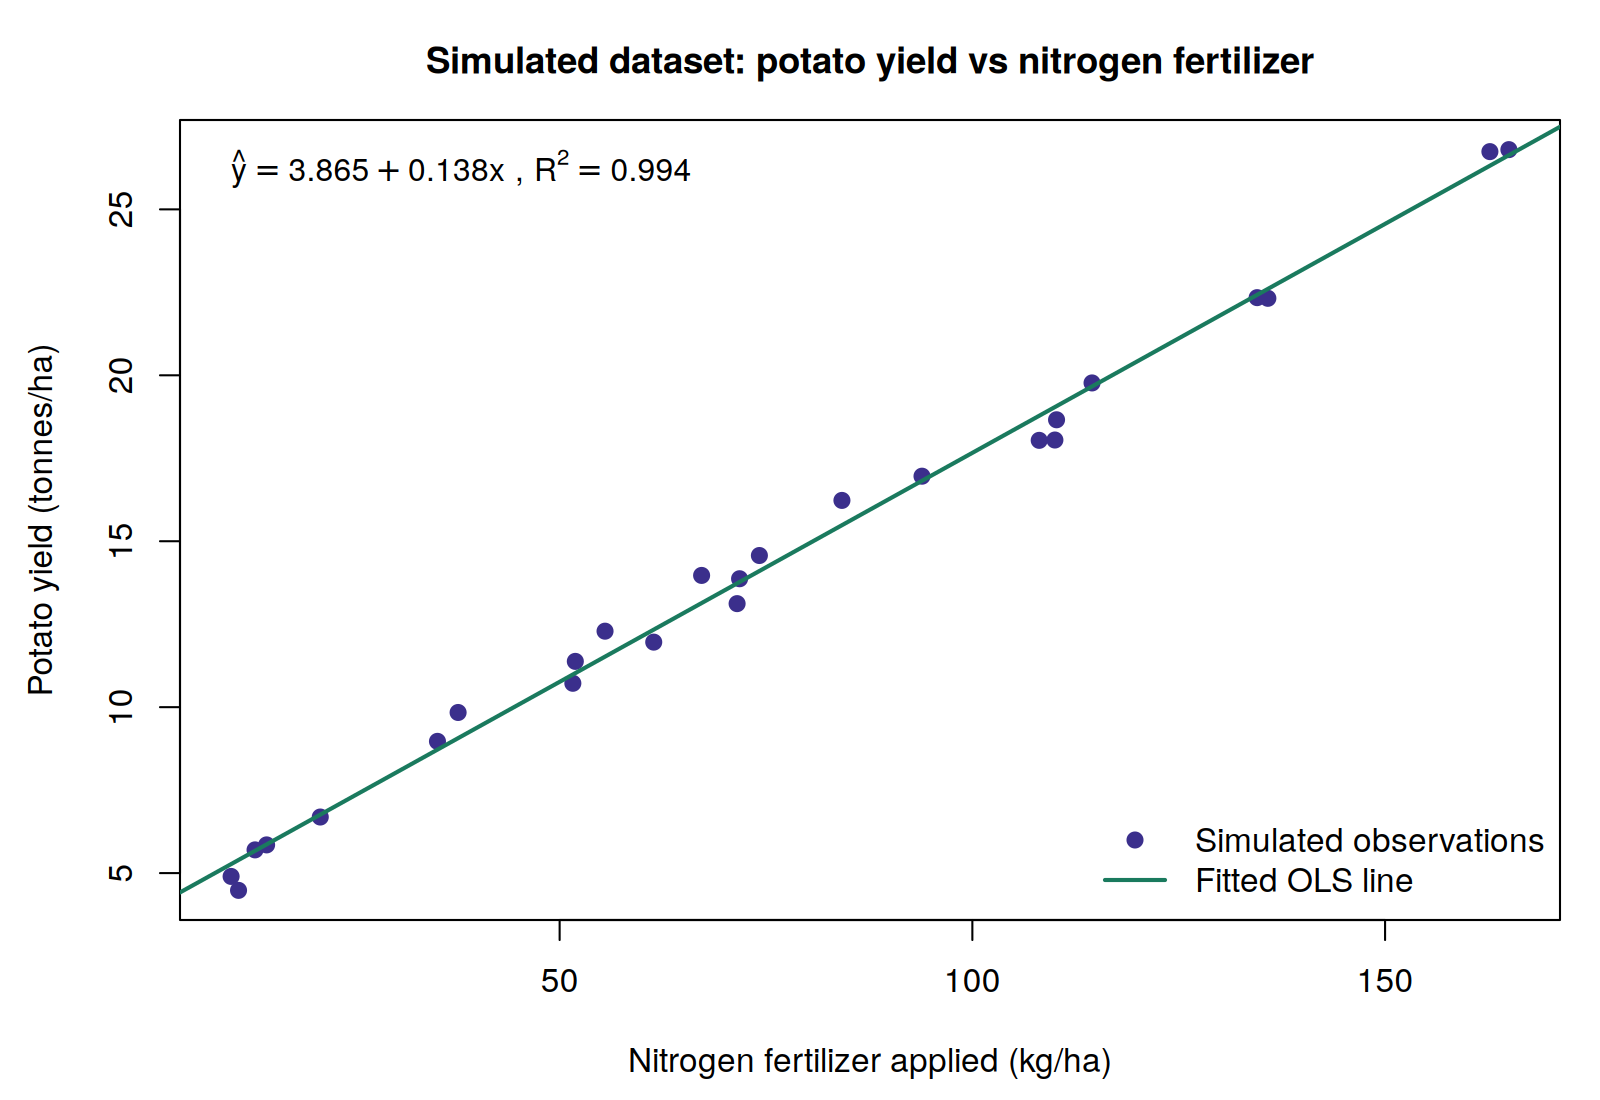
\includegraphics[width=0.85\linewidth]{assets/application-ols-simulation.png}
\end{screenshot}
\captionof{figure}{Simulated nitrogen-yield dataset with the fitted OLS line.}

The fitted line, $\hat y = 3.865+0.138x$ with $R^2=0.994$, lands almost exactly on the $\hat y = 3.94+0.139x$, $R^2=0.99$ seen in the exploration-phase figure, confirming that the by-hand normal equations, the matrix form $\hat\beta=(X^\top X)^{-1}X^\top Y$, and R's own \texttt{lm()} solver all converge on the same answer.


\chapter{Different Types of Response Variables}

\Exploration

To get a feel for this topic before formalising anything, I watched a video on different types of response variables on YouTube.

\begin{screenshot}
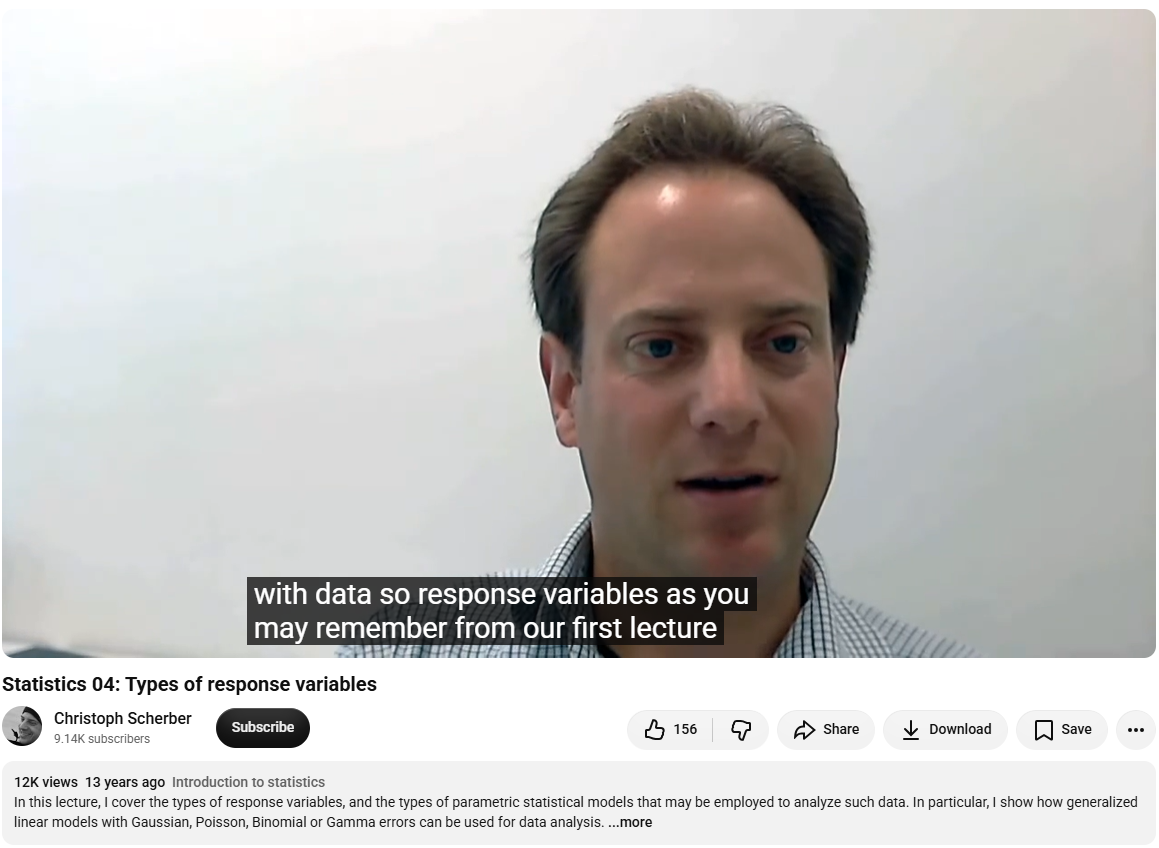
\includegraphics[width=\linewidth]{assets/exploration-response-variables-video.png}
\end{screenshot}
\captionof{figure}{Types of response variables, from a YouTube lecture \citep{scherber_response_variables}.}
\explorationsource{Scherber, C., \textit{Statistics 04: Types of Response Variables}, YouTube.}

From this video I picked up a few things about response variables:

\begin{enumerate}
\item A response variable is what we usually put on the $y$-axis, and it's dependent on the explanatory variables on the $x$-axis.
\item A response variable is the main output we're interested in, the main reason the model was built in the first place.
\item Since it's our aim, we can aim to do many different things with it: measure, count, partition. Because of this, we end up with different types of response variables, each carrying its own distribution.
\end{enumerate}

We move on to the Cognition phase, where these intuitions get sorted into a proper table.

\Cognition

Now, to build solid cognitive pillars on top of that intuitive background, the table below sets out the different response variables and the distributions that typically go with them.

\begin{table}[h]
\centering
\renewcommand{\arraystretch}{1.4}
\begin{tabular}{p{3.6cm}p{2.6cm}p{2cm}p{3.2cm}}
\toprule
\textbf{Outcome} & \textbf{Distribution} & \textbf{Typical Link} & \textbf{Form of $\eta$} \\
\midrule
Continuous, symmetric, can be positive or negative & Normal & Identity & $\mu$ \\
Binary (yes/no), proportion out of $n$ trials & Binomial (Bernoulli) & Logit & $\log\left(\dfrac{\pi}{1-\pi}\right)$ \\
Count, no fixed upper limit & Poisson & Log & $\log(\mu)$ \\
Count, overdispersed ($\operatorname{Var} \gg \operatorname{Mean}$) & Negative Binomial & Log & $\log(\mu)$ \\
Continuous, positive, right-skewed & Gamma & Log or Inverse & $\log(\mu)$ \\
\bottomrule
\end{tabular}
\caption{Common response variable types, their typical distributions, and typical link functions.}
\end{table}

$\eta$ is the same idea no matter which distribution is in play,
\begin{mathbox}
\[
\eta = \beta_0 + \beta_1 x_1 + \beta_2 x_2 + \cdots + \beta_k x_k
\]
\end{mathbox}
It's just the linear combination of explanatory variables. The link function is what connects $\eta$ to the mean of the outcome's distribution.

\begin{figure}[h]
\centering
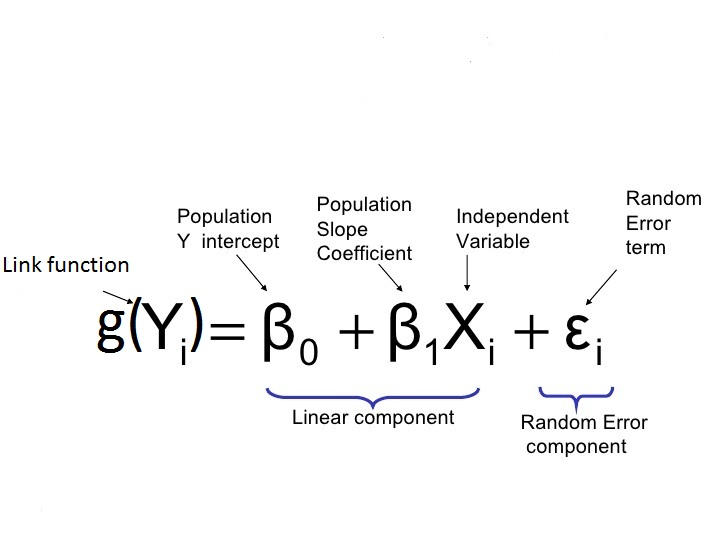
\includegraphics[width=0.7\linewidth]{assets/cognition-link-function-diagram.jpeg}
\caption{How a link function sits inside the linear predictor \citep{chandan_logistic}.}
\end{figure}

\Reflection

So, to reflect on this, let's work through a couple of scenarios and decide, each time, what distribution the response follows, then write out the linear component and link function to get some firsthand decision-making experience.

\subsection*{Scenario 1: Loan Default}
A bank wants to predict whether a customer defaults on a loan (yes/no), using annual income, credit score, and number of existing loans.

\begin{itemize}
\item \textbf{Outcome ($Y$):} Default (1 = yes, 0 = no).
\item \textbf{Explanatory ($X$'s):} Income, credit score, number of existing loans.
\item \textbf{Distribution:} Binomial (Bernoulli, one trial per customer).
\item \textbf{Link:} Logit.
\end{itemize}
\begin{mathbox}
\[
\eta = \beta_0 + \beta_1(\text{income}) + \beta_2(\text{credit score}) + \beta_3(\text{number of loans})
\]
\end{mathbox}

\subsection*{Scenario 2: Traffic Accidents}
\begin{itemize}
\item \textbf{Outcome ($Y$):} Number of accidents per month at an intersection (count, no natural cap).
\item \textbf{Explanatory ($X$'s):} Traffic volume, traffic light (yes/no), speed limit.
\item \textbf{Distribution:} Poisson.
\item \textbf{Link:} Log.
\end{itemize}
\begin{mathbox}
\[
\eta = \beta_0 + \beta_1(\text{traffic volume}) + \beta_2(\text{traffic light}) + \beta_3(\text{speed limit})
\]
\end{mathbox}

\begin{questionbox}[: Why do we bother with different types of response variables?]
As usual, to get at the real reason we generalise linear models, it helps to go back to why we make models at all: to get some outcome. In the simple linear model that outcome is usually just a continuous real number, typically unbounded except in special cases. But suppose we want to make inference on the proportion of rabbits with a certain deformity. Our outcome is now a binomial response, since each rabbit either has the deformity or doesn't, but what we actually want is the percentage of rabbits that get it. We still want to use a linear model to describe this, but for that to work we need to generalise the linear model using a link function, one that connects our binary outcomes to a linear predictor that gives back a continuous real number.
\end{questionbox}


\chapter{The Language of GLMs}

\Exploration

If GLMs were a demographic of people, they would have their own language. But to understand the language of these people, we first need to understand why we want to speak to them in the first place: what they eat, what they stand for, and their purpose in the grand scheme of things. Okay, enough of the analogy, before we dive into the boring definitions, let's take a moment to examine the actual aim of GLMs.

\textbf{Aim:} As simply as possible, the aim of GLMs is to know how a bunch of $X$'s affect a $Y$. That's the simplest definition.

Let's step into a time machine. This time machine takes us to 1972, when John Nelder and Robert Wedderburn formulated a framework for unifying various other statistical models, e.g.\ linear regression, logistic regression, and Poisson regression \citep{nelder1972}, along with a neat solution for maximum likelihood estimation known as the iteratively reweighted least squares method.

As we have already established intuitively, OLS predicts the expected value of a random variable $Y$ as a linear combination of a set of observed values (a ``bunch of $X$'s''), also known as predictors. We can make a few assumptions based on this:

\begin{enumerate}
\item A constant change in a predictor leads to a constant change in the response.
\item In the case of OLS, these assumptions hold when the response can vary indefinitely in both directions, i.e.\ it follows the pattern of a normal distribution.
\item However, when the response doesn't follow this pattern, we can use transformations to make it follow that pattern.
\item When these transformations are not sufficient, we employ the use of GLMs.
\end{enumerate}

\begin{screenshot}
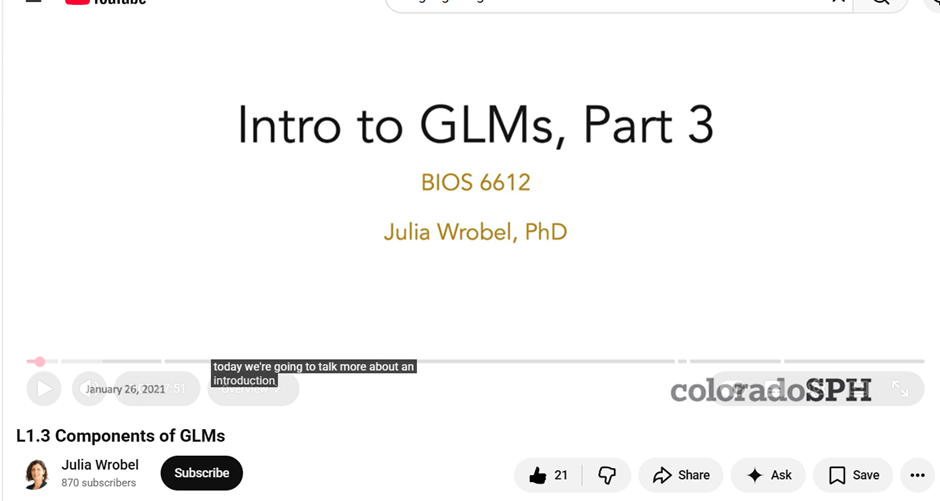
\includegraphics[width=0.75\linewidth]{assets/exploration-glm-components-video.png}
\end{screenshot}
\captionof{figure}{Components of GLMs, from a YouTube lecture \citep{wrobel_components}.}
\explorationsource{Wrobel, J. (2021, January 25), \textit{L1.3 Components of GLMs}, YouTube.}

Quick summary of this framework from a YouTube video I watched, before we dive into more definitions: assume that a known function of $\mu_i$ is related linearly to covariates,
\begin{mathbox}
\[
g(\mu_i) = \eta_i = x_i^\top\beta
\]
\end{mathbox}
Then:
\begin{enumerate}
\item $g$ = link function: links the linear predictor with the mean of the outcome.
\item We assume independence of $Y_i$.
\item The linearity assumption now applies to $\eta_i$, which need not equal $\mu_i$.
\item $X$ is treated as fixed.
\end{enumerate}

\Cognition

This chapter collects, in one place, the vocabulary used throughout the rest of the portfolio. Later chapters build on these terms without redefining them.

\term{Generalised Linear Model}
A generalised linear model is a generalisation of linear regression that is more versatile. The GLM generalises linear regression by connecting the linear model to the response variable via a link function, and by permitting the variance of each measurement to be a function of its predicted value \citep{nelder1972,mccullagh1989}.

\term{Log-linear Model}
A log-linear model is a mathematical model that allows for the application of potential multivariate linear regression by taking the form of a function whose logarithm equals a linear combination of the model's parameters:
\begin{mathbox}
\[
\exp\left\{c + \sum_i w_i f_i(X)\right\}
\]
\end{mathbox}
where $f_i(X)$ are functions of the vector of values $X$, and $c$ and $w_i$ are model parameters. Taking the natural log of this gives a linear combination that can be worked with directly \citep{agresti2015}.

\begin{defbox}[: Exponential Family]
An exponential family is a parametric set of probability distributions with the form
\[
f_X(x \mid \theta) = h(x)\exp\left\{\eta(\theta)\cdot T(x) - A(\theta)\right\}
\]
where $h(x)$ is non-negative and known, and $\eta(\theta)$, $T(x)$, $A(\theta)$ are known as well \citep{mccullagh1989,wikipedia_glm}.
\end{defbox}

\begin{defbox}[: One-Parameter Exponential Family]
A one-parameter exponential family is a special case of the exponential family in which the distribution depends on a single scalar parameter $\theta$, and its probability density (or mass) function can be written
\[
f(y;\theta) = \exp\left\{a(y)\,b(\theta) + c(\theta) + d(y)\right\}
\]
where $a(y)$ is the sufficient statistic, $b(\theta)$ is the natural (canonical) parameter, $c(\theta)$ is the log-partition function ensuring the density normalises to one, and $d(y)$ is the base measure, a term depending on $y$ alone. This form underlies several of the standard distributions used in GLMs, such as the Binomial and Poisson, for which the dispersion parameter is fixed at 1 \citep{taylor_nd}.
\end{defbox}

\term{Link Function}
A link function links the predicted mean of the response variable $\mu$ to the linear predictor $\eta$ in a GLM:
\begin{mathbox}
\[
g(\mu) = \eta = X\beta = \beta_0+\beta_1 x_1+\beta_2 x_2+\cdots+\beta_n x_n, \qquad \mu = g^{-1}(X\beta)
\]
\end{mathbox}
When $g$ is chosen such that the linear predictor equals the natural parameter of the distribution, it is called a canonical link function for that distribution, e.g.\ the logit link for the Binomial, or the log link for the Poisson \citep{dobson2018}.

\term{Transposed Matrix}
For any matrix $A$ with dimensions $m\times n$, the transpose $A^\top$ is the $n\times m$ matrix obtained by swapping its rows and columns: $(A^\top)_{ij} = A_{ji}$. Transposition is central to GLM estimation: for a design matrix $X$ and coefficient vector $\beta$, the normal equations used to estimate $\beta$ take the form $\hat\beta = (X^\top X)^{-1}X^\top y$, reflecting the orthogonality condition $X^\top(y-\mu(\beta))=0$ that arises from likelihood theory in GLMs \citep{casella2002}.

\term{Transposed Vector}
A transposed vector is a vector whose rows and columns have been flipped, so a column vector becomes a row vector or vice versa. For a column vector of covariates $x_i$ and column vector of coefficients $\beta$, $x_i^\top\beta = x_{i1}\beta_1+x_{i2}\beta_2+\cdots+x_{ip}\beta_p$, which is precisely the linear predictor $\eta_i$, a single scalar value \citep{casella2002}.

\term{Linear Predictor}
Denoted $X\beta$, this is the linear combination of covariates and regression coefficients that links the explanatory variables to the response distribution's mean through the link function \citep{dobson2018}.

\term{Parameters}
Quantities that characterise a probability distribution or a statistical model, whose values determine its shape, location, or scale. In a GLM, parameters include the regression coefficients ($\beta$), the dispersion parameter ($\phi$), and any other parameter implicit in the chosen distribution \citep{casella2002}.

\term{Sufficiency}
A property of a statistic whereby it captures all the information in a sample relevant to estimating a parameter, such that no other statistic calculated from the same sample provides additional information about that parameter \citep{casella2002}.

\term{Sufficient Statistic $a(y)$}
The statistic $a(y)$ that satisfies the property of sufficiency for a parameter. In exponential family notation, it is the function of the data multiplied by the natural parameter in the exponent. In many cases $a(y)=y$, and the distribution is then said to be in canonical form \citep[p.~2]{nowak_nd}.

\term{Natural Parameter $b(\theta)$}
Also called the canonical parameter, this is the parameter that appears in the exponent of a distribution written in exponential family form. It is the parameter through which the linear predictor connects to the distribution when a canonical link function is used \citep{mccullagh1989}.

\term{Log-partition Function $c(\theta)$}
Also called the cumulant function or normalising function, this ensures the exponential family density integrates (or sums) to one. Its derivatives generate the moments of the sufficient statistic: the first derivative gives the mean, the second gives the variance \citep{mccullagh1989}.

\term{Base Measure $d(y)$}
The component of the exponent that depends on $y$ alone, independent of $\theta$. It functions as a normalising term ensuring the density integrates to 1 \citep{mccullagh1989}.

\term{Dispersion Parameter}
A parameter, denoted $\phi$, that scales the variance of the response distribution independently of its mean. It reflects variability beyond what is explained by the mean-variance relationship of the chosen distribution. In the one-parameter exponential family form the dispersion parameter is fixed at 1 \citep{dobson2018}.

\term{Score Function}
The first derivative of the log-likelihood function with respect to the parameter(s) of interest. Setting the score function equal to zero and solving yields the maximum likelihood estimate \citep{casella2002}.

\term{Maximum Likelihood Estimates}
The parameter values that maximise the likelihood function, i.e.\ the values that make the observed data most probable under the assumed model. In GLMs, MLEs for $\beta$ are typically obtained via iterative methods such as Iteratively Reweighted Least Squares (IRLS), since closed-form solutions rarely exist outside the Gaussian case \citep{casella2002}.

\term{Canonical Form}
A distribution is said to be in canonical form when its sufficient statistic $a(y)$ equals $y$ itself, in which case the natural parameter is also called the canonical parameter \citep{mccullagh1989}.

\term{Logit}
The canonical link function for the binomial distribution, defined as the log-odds:
\begin{mathbox}
\[
g(\mu) = \log\left(\frac{\mu}{1-\mu}\right)
\]
\end{mathbox}
It maps probabilities bounded between 0 and 1 onto the entire real line, making it suitable for linear modelling \citep{dobson2018}.

\term{Probit}
A link function defined as the inverse of the standard normal cumulative distribution function, $g(\mu) = \Phi^{-1}(\mu)$. Commonly used for binary response models as an alternative to the logit link \citep{dobson2018}.

\term{Nuisance Parameter}
A parameter in a statistical model that is not of primary interest but must be accounted for in order to correctly estimate the parameters that are of interest. In many GLMs, the dispersion parameter is treated as a nuisance parameter \citep{casella2002}.

\Reflection
\tbc

% ================= PART II =================
\part{The Mathematics Behind GLMs}

\chapter{The Exponential Family}

\Exploration
\tbc

\Cognition

\section{Definition and Properties}

A probability distribution belongs to the exponential family if its density (or mass) function can be written in the general form
\begin{mathbox}
\[
f_X(x\mid\theta) = h(x)\exp\left\{\eta(\theta)\cdot T(x) - A(\theta)\right\}
\]
\end{mathbox}
Here $h(x)$ is a known, non-negative function of the data alone, while $\eta(\theta)$, $T(x)$ and $A(\theta)$ are known functions governing the natural parameter, the sufficient statistic, and the normalising term respectively \citep{mccullagh1989}. In this general version $\theta$ may be a vector and $T(x)$ a vector of sufficient statistics, so this is sometimes called the multi-parameter or full exponential family.

For GLMs, though, what matters is the one-parameter exponential family, since this is the restricted form underlying the standard GLM distributions: Binomial, Poisson, Normal, and Gamma. Restricting $\theta$ to a scalar and writing the exponent as a sum rather than a dot product gives the working form used throughout this portfolio:
\begin{mathbox}
\[
f(y;\theta) = \exp\left\{a(y)\,b(\theta) + c(\theta) + d(y)\right\}
\]
\end{mathbox}
Matching the terms defined in Part I:
\begin{itemize}
\item $a(y)$ is the sufficient statistic: the function of the data that gets multiplied by the natural parameter.
\item $b(\theta)$ is the natural (canonical) parameter, the function of $\theta$ through which the linear predictor will eventually connect to the distribution.
\item $c(\theta)$ is the log-partition function, which guarantees $f(y;\theta)$ integrates (or sums) to one over its support.
\item $d(y)$ is the base measure, the leftover piece depending on $y$ alone, with no $\theta$ in it.
\end{itemize}
What makes this form useful is the separation it forces between data and parameter. $y$ and $\theta$ never appear multiplied together except through the product $a(y)\,b(\theta)$; everything else involving $y$ sits in $d(y)$, and everything else involving $\theta$ sits in $c(\theta)$. This separation is also what makes $a(y)$ sufficient in the first place: once $a(y)$ is known, nothing more about $y$ is needed to work out how the likelihood depends on $\theta$.

A distribution is in canonical form when $a(y)=y$. In that case $b(\theta)$ is called the canonical parameter, and, as covered later when link functions are discussed, the link function that sets the linear predictor equal to $b(\theta)$ directly is the canonical link for that distribution.

$c(\theta)$ is worth dwelling on a little longer, because it isn't really a free choice, it's forced by the requirement that $f(y;\theta)$ be a valid density. Given $a(y)$, $b(\theta)$ and $d(y)$, normalisation requires
\begin{mathbox}
\[
\int \exp\{a(y)\,b(\theta)+d(y)\}\,dy = \exp\{-c(\theta)\}
\]
\end{mathbox}
(or the equivalent sum in the discrete case), so $c(\theta)$ ends up completely determined by the rest of the exponent. This is also why $c(\theta)$ is called the cumulant function: differentiating it with respect to $\theta$ generates the moments of $a(y)$. Under the canonical parameterisation, $\mathbb{E}[a(Y)] = -c'(\theta)$ and $\operatorname{Var}[a(Y)] = -c''(\theta)$, a fact that becomes useful once the mean-variance relationships for individual GLM distributions are worked out further on.

\subsection*{Proof: $c(\theta)$ as the Cumulant (Normalising) Function}
The claim above, that $c(\theta)$ is forced by normalisation rather than being a free choice, is not asserted without justification; it follows directly from requiring $f(y;\theta)$ to be a valid density. The derivation below is a proof of that result.

Since $f(y;\theta)$ is a probability density (or mass) function, it must integrate, or sum in the discrete case, to 1:
\begin{mathbox}
\[
\int f(y;\theta)\,dy = 1
\]
\end{mathbox}
Substituting the one-parameter exponential family form gives
\begin{mathbox}
\[
\int \exp\{a(y)b(\theta)+c(\theta)+d(y)\}\,dy = 1
\]
\end{mathbox}
Since $c(\theta)$ does not depend on $y$, it can be factored out of the integral using $\exp\{A+B\}=\exp\{A\}\cdot\exp\{B\}$:
\begin{mathbox}
\[
\exp\{c(\theta)\}\int \exp\{a(y)b(\theta)+d(y)\}\,dy = 1
\]
\end{mathbox}
Dividing both sides by the remaining integral isolates $\exp\{c(\theta)\}$:
\begin{mathbox}
\[
\exp\{c(\theta)\} = \left(\int \exp\{a(y)b(\theta)+d(y)\}\,dy\right)^{-1}
\]
\end{mathbox}
Taking the logarithm of both sides,
\begin{mathbox}
\[
\log\left[\exp\{c(\theta)\}\right] = \log\left[\left(\int \exp\{a(y)b(\theta)+d(y)\}\,dy\right)^{-1}\right]
\]
\end{mathbox}
which simplifies, using $\log(x^{-1}) = -\log(x)$, to
\begin{mathbox}
\[
\therefore\ c(\theta) = -\log\int \exp\{a(y)b(\theta)+d(y)\}\,dy
\]
\end{mathbox}
Equivalently, moving the negative sign across gives
\begin{mathbox}
\[
-c(\theta) = \log\int \exp\{a(y)b(\theta)+d(y)\}\,dy
\]
\end{mathbox}
and exponentiating both sides recovers the normalisation identity stated above:
\begin{mathbox}
\[
\exp\{-c(\theta)\} = \int \exp\{a(y)b(\theta)+d(y)\}\,dy
\]
\end{mathbox}
This confirms that, given $a(y)$, $b(\theta)$, and $d(y)$, the function $c(\theta)$ is not an independent modelling choice but is fully determined by the requirement that the density integrate to one. $\blacksquare$

\section{Why the Exponential Family Matters}

\subsection*{Toward a Unified Framework}
Nelder and Wedderburn's insight, in 1972, was that a wide range of these non-normal response distributions, Binomial, Poisson, Gamma, and Normal among them, could all be written in the same one-parameter exponential family form introduced above. Once a distribution is expressed that way, the same general machinery (score equations, Fisher information, iteratively reweighted least squares) can be used to estimate its parameters, regardless of which member of the family is in play. The generalised linear model is precisely this: a linear predictor for the mean, exactly as in the classical linear model, combined with a chosen distribution from the exponential family and a link function that connects the mean of that distribution to the linear predictor, allowing the connection to be nonlinear (such as the log-odds link mentioned above) where the data demand it.

This is why the exponential family matters so much to GLM theory. It is not simply a convenient algebraic form, it is the structural bridge that lets the well-understood machinery of the linear model be reused, almost unchanged in spirit, across an entire class of response distributions that would otherwise each require their own separate theory \citep{nelder1972,dobson2018}.

\Reflection
\tbc

\Application
\tbc


\chapter{Building the Exponential Family}

\Exploration
\tbc

\Cognition

\section{Normal Distribution}
The Normal distribution, also known as the Gaussian distribution, is a continuous probability distribution for a real-valued random variable. It occupies a central place in statistics, largely because of the Central Limit Theorem: the average of many statistically independent observations of a random variable, provided that variable has a finite mean and variance, converges to a normal distribution as the number of observations grows large. Consequently, physical quantities that arise as the sum of many independent processes, such as height or measurement error, tend to be approximately normally distributed \citep{casella2002}.

\subsection*{Probability Density Function}
\begin{mathbox}
\[
f(y;\mu) = \frac{1}{(2\pi\sigma^2)^{1/2}}\exp\left\{-\frac{(y-\mu)^2}{2\sigma^2}\right\}
\]
\end{mathbox}

\subsection*{Rewriting in One-Parameter Exponential Form}
Taking logs of both sides gives
\begin{mathbox}
\[
\log f(y;\mu) = -\frac{1}{2}\log(2\pi\sigma^2) - \frac{(y-\mu)^2}{2\sigma^2}
\]
\end{mathbox}
Expanding the square in the exponent separates the terms depending on $y$ alone, $\mu$ alone, and both together:
\begin{mathbox}
\[
\log f(y;\mu) = -\frac{1}{2}\log(2\pi\sigma^2) - \frac{y^2}{2\sigma^2} + \frac{y\mu}{\sigma^2} - \frac{\mu^2}{2\sigma^2}
\]
\end{mathbox}
Exponentiating both sides and grouping terms according to the one-parameter exponential family form $f(y;\theta)=\exp\{a(y)b(\theta)+c(\theta)+d(y)\}$ then gives
\begin{mathbox}
\[
f(y;\mu) = \exp\left\{y\cdot\frac{\mu}{\sigma^2} - \frac{\mu^2}{2\sigma^2} - \left[\frac{1}{2}\log(2\pi\sigma^2)+\frac{y^2}{2\sigma^2}\right]\right\}
\]
\end{mathbox}
so that, with $\theta=\mu$,
\begin{mathbox}
\[
a(y)=y,\quad b(\mu)=\frac{\mu}{\sigma^2},\quad c(\mu)=-\frac{\mu^2}{2\sigma^2},\quad d(y)=-\left[\frac{1}{2}\log(2\pi\sigma^2)+\frac{y^2}{2\sigma^2}\right]
\]
\end{mathbox}
Since $a(y)=y$, the Normal distribution is in canonical form. When the dispersion is treated as fixed, as in the one-parameter form used throughout this portfolio, so that $\sigma^2=1$, $b(\mu)$ reduces to $\mu$ itself, meaning the natural parameter coincides with the mean. The canonical link for the Normal distribution is therefore the identity link $g(\mu)=\mu$, which is consistent with how the mean is modelled directly in the classical linear model discussed in Part III.

\subsection*{Proof: Normalising Term $c(\mu)$}
The value of $c(\mu)$ stated above is not an arbitrary choice; it follows from the general normalisation identity proved above, applied here with $a(y)=y$, $b(\mu)=\mu/\sigma^2$, and $d(y)=-\left[\frac{1}{2}\log(2\pi\sigma^2)+y^2/(2\sigma^2)\right]$.

Starting from the identity $\exp\{-c(\mu)\} = \int\exp\{a(y)b(\mu)+d(y)\}\,dy$ and substituting these terms gives
\begin{mathbox}
\[
\exp\{-c(\mu)\} = \int \exp\left\{\frac{y\mu}{\sigma^2}-\frac{y^2}{2\sigma^2}-\frac{1}{2}\log(2\pi\sigma^2)\right\}dy
\]
\end{mathbox}
Since the last term does not depend on $y$, it can be pulled outside the integral:
\begin{mathbox}
\[
\exp\{-c(\mu)\} = \frac{1}{\sqrt{2\pi\sigma^2}}\int \exp\left\{\frac{y\mu}{\sigma^2}-\frac{y^2}{2\sigma^2}\right\}dy
\]
\end{mathbox}
Completing the square in the remaining exponent, since $\dfrac{y\mu}{\sigma^2}-\dfrac{y^2}{2\sigma^2} = -\dfrac{(y-\mu)^2}{2\sigma^2}+\dfrac{\mu^2}{2\sigma^2}$, gives
\begin{mathbox}
\[
\exp\{-c(\mu)\} = \frac{1}{\sqrt{2\pi\sigma^2}}\exp\left\{\frac{\mu^2}{2\sigma^2}\right\}\int\exp\left\{-\frac{(y-\mu)^2}{2\sigma^2}\right\}dy
\]
\end{mathbox}
The remaining integral is the standard Gaussian integral, which evaluates to $\sqrt{2\pi\sigma^2}$, so this reduces to
\begin{mathbox}
\[
\exp\{-c(\mu)\} = \frac{1}{\sqrt{2\pi\sigma^2}}\cdot\exp\left\{\frac{\mu^2}{2\sigma^2}\right\}\cdot\sqrt{2\pi\sigma^2} = \exp\left\{\frac{\mu^2}{2\sigma^2}\right\}
\]
\end{mathbox}
Equating exponents and solving for $c(\mu)$ therefore gives
\begin{mathbox}
\[
-c(\mu) = \frac{\mu^2}{2\sigma^2} \implies \therefore\ c(\mu) = -\frac{\mu^2}{2\sigma^2}\quad \blacksquare
\]
\end{mathbox}
This confirms that $c(\mu)$ is forced by the same normalisation constraint established generally above, worked through here with the specific $a(y)$ and $d(y)$ that arise from the Normal density.

\section{Binomial Distribution}
The Binomial distribution is a discrete probability distribution for the number of successes in a sequence of $n$ independent trials, each with a boolean outcome, success or failure, where success occurs with probability $p$ and failure with probability $1-p$, since the two outcomes must sum to 1. The special case $n=1$ is the Bernoulli distribution, so the Binomial can be thought of as a generalisation of a sequence of Bernoulli trials \citep{casella2002}.

\subsection*{Probability Mass Function}
\begin{mathbox}
\[
f(y;n,p) = \binom{n}{y}p^y(1-p)^{n-y}, \qquad y=0,1,\dots,n
\]
\end{mathbox}

\subsection*{Rewriting in One-Parameter Exponential Form}
Taking logs of both sides gives
\begin{mathbox}
\[
\log f(y;n,p) = \log\binom{n}{y} + y\log(p) + (n-y)\log(1-p)
\]
\end{mathbox}
Expanding the last term and collecting everything that multiplies $y$ separates the exponent into a piece linear in $y$ and a piece that does not depend on $y$ at all:
\begin{mathbox}
\[
\log f(y;n,p) = y\log(p) - y\log(1-p) + n\log(1-p) + \log\binom{n}{y} = y\log\left(\frac{p}{1-p}\right) + n\log(1-p) + \log\binom{n}{y}
\]
\end{mathbox}
Exponentiating both sides and grouping terms according to $f(y;\theta) = \exp\{a(y)b(\theta)+c(\theta)+d(y)\}$ then gives
\begin{mathbox}
\[
f(y;n,p) = \exp\left\{y\log\left(\frac{p}{1-p}\right) + n\log(1-p) + \log\binom{n}{y}\right\}
\]
\end{mathbox}
so that, with $\theta=p$,
\begin{mathbox}
\[
a(y)=y,\quad b(p)=\log\left(\frac{p}{1-p}\right),\quad c(p) = n\log(1-p),\quad d(y)=\log\binom{n}{y}
\]
\end{mathbox}
Since $a(y)=y$, the Binomial distribution is in canonical form, and $b(p)$ is its canonical parameter. Because $b(p) = \log\left(\frac{p}{1-p}\right)$ is exactly the logit function defined in Part II, the canonical link for the Binomial distribution is the logit link, which is why logistic regression models the log-odds of success as a linear predictor rather than the probability itself.

\subsection*{Proof: Normalising Term $c(p)$}
The value of $c(p)$ stated above is not an arbitrary choice; it follows from the general normalisation identity proved above, applied here with $a(y)=y$, $b(p)=\log\left(\frac{p}{1-p}\right)$, and $d(y)=\log\binom{n}{y}$. Since the Binomial distribution is discrete, the identity holds with a sum in place of an integral.

Starting from $\exp\{-c(p)\} = \sum_{y=0}^n \exp\{a(y)b(p)+d(y)\}$ and substituting these terms gives
\begin{mathbox}
\[
\exp\{-n\log(1-p)\} = \sum_{y=0}^n \exp\left\{y\log\left(\frac{p}{1-p}\right) + \log\binom{n}{y}\right\}
\]
\end{mathbox}
Evaluating the exponent on the right, using $\exp\{A+B\}=\exp\{A\}\exp\{B\}$,
\begin{mathbox}
\[
\exp\left\{y\log\left(\frac{p}{1-p}\right) + \log\binom{n}{y}\right\} = \exp\left\{y\log\left(\frac{p}{1-p}\right)\right\}\cdot\exp\left\{\log\binom{n}{y}\right\} = \left(\frac{p}{1-p}\right)^y\binom{n}{y}
\]
\end{mathbox}
so the right-hand side becomes
\begin{mathbox}
\[
\sum_{y=0}^n \left(\frac{p}{1-p}\right)^y\binom{n}{y} = \left(1+\frac{p}{1-p}\right)^n
\]
\end{mathbox}
by the Binomial theorem. Simplifying the base,
\begin{mathbox}
\[
\left(1+\frac{p}{1-p}\right)^n = \left(\frac{1-p+p}{1-p}\right)^n = \left(\frac{1}{1-p}\right)^n = (1-p)^{-n}
\]
\end{mathbox}
This matches the left-hand side exactly, since
\begin{mathbox}
\[
\exp\{-n\log(1-p)\} = (1-p)^{-n}
\]
\end{mathbox}
Equating both sides and taking logs confirms the identity holds:
\begin{mathbox}
\[
\log\left[\exp\{-n\log(1-p)\}\right] = \log\left[(1-p)^{-n}\right] \implies -n\log(1-p) = -n\log(1-p) \quad\blacksquare
\]
\end{mathbox}
This proves that $c(p) = n\log(1-p)$ is the function that makes $\sum_{y=0}^n f(y;n,p) = 1$.

\section{Poisson Distribution}
The Poisson distribution is a discrete probability distribution that expresses the probability of a number of events occurring in a fixed interval of time (or space), given that these events occur with a known constant mean rate and independently of the time since the last event \citep{casella2002}.

\subsection*{Probability Mass Function}
\begin{mathbox}
\[
f(y;\lambda) = \frac{\lambda^y e^{-\lambda}}{y!}, \qquad \lambda = \text{rate parameter},\ y=0,1,2,\dots
\]
\end{mathbox}

\subsection*{Rewriting in One-Parameter Exponential Form}
Taking logs of both sides gives
\begin{mathbox}
\[
\log f(y;\lambda) = y\log(\lambda) - \lambda - \log(y!)
\]
\end{mathbox}
This is already separated into a piece linear in $y$, a piece depending on $\lambda$ alone, and a piece depending on $y$ alone, so exponentiating and grouping terms according to $f(y;\theta)=\exp\{a(y)b(\theta)+c(\theta)+d(y)\}$ gives
\begin{mathbox}
\[
f(y;\lambda) = \exp\left\{y\log(\lambda) - \lambda - \log(y!)\right\}
\]
\end{mathbox}
so that, with $\theta=\lambda$,
\begin{mathbox}
\[
a(y)=y,\quad b(\lambda)=\log(\lambda),\quad c(\lambda) = -\lambda,\quad d(y) = -\log(y!)
\]
\end{mathbox}
Since $a(y)=y$, the Poisson distribution is in canonical form, and $b(\lambda)=\log(\lambda)$ is its canonical parameter. The canonical link for the Poisson distribution is therefore the log link, $g(\mu)=\log(\mu)$, which is why Poisson regression models the log of the mean count as a linear predictor.

\subsection*{Proof: Normalising Term $c(\lambda)$}
The value of $c(\lambda)$ stated above is not an arbitrary choice; it follows from the general normalisation identity proved above, applied here with $a(y)=y$, $b(\lambda)=\log(\lambda)$, and $d(y)=-\log(y!)$. Since the Poisson distribution is discrete with unbounded support $y=0,1,2,\dots$, the identity holds with an infinite sum in place of an integral.

Starting from $\exp\{-c(\lambda)\} = \sum_{y=0}^{\infty}\exp\{a(y)b(\lambda)+d(y)\}$ and substituting these terms gives
\begin{mathbox}
\[
\exp\{-(-\lambda)\} = \sum_{y=0}^{\infty}\exp\left\{y\log(\lambda) - \log(y!)\right\}
\]
\end{mathbox}
Decomposing the exponent on the right using exponential laws,
\begin{mathbox}
\[
\exp\left\{y\log(\lambda) - \log(y!)\right\} = \frac{\exp\{y\log(\lambda)\}}{\exp\{\log(y!)\}} = \frac{\lambda^y}{y!}
\]
\end{mathbox}
so the identity becomes
\begin{mathbox}
\[
\exp\{\lambda\} = \sum_{y=0}^{\infty}\frac{\lambda^y}{y!}
\]
\end{mathbox}
The right-hand side is exactly the Maclaurin series expansion of the exponential function, which is known to equal $e^\lambda$:
\begin{mathbox}
\[
\sum_{y=0}^{\infty}\frac{\lambda^y}{y!} = e^\lambda = \exp\{\lambda\}
\]
\end{mathbox}
Equating both sides confirms the identity holds,
\begin{mathbox}
\[
\exp\{\lambda\} = \exp\{\lambda\} \quad\blacksquare
\]
\end{mathbox}
This proves that $c(\lambda) = -\lambda$ is the function that makes $\sum_{y=0}^{\infty} f(y;\lambda) = 1$.

\section{Gamma Distribution}
The Gamma distribution is a two-parameter family of continuous probability distributions with many applications across fields such as econometrics and Bayesian statistics \citep{casella2002}. In econometrics, the $(\alpha,\theta)$ shape-scale parameterisation is commonly used to model waiting times, such as time until failure, where it often takes the form of a special case of the Gamma distribution, the Erlang distribution, for integer $\alpha$. In Bayesian statistics, the parameterisation takes the form $(\alpha,\beta)$, with $\beta=1/\theta$ the rate parameter, and the Gamma distribution is widely used as a conjugate prior for several inverse scale parameters, which facilitates analytical tractability in posterior computations. In GLMs, it is more convenient to work with a mean-shape parameterisation, writing the Gamma distribution in terms of its mean $\mu$ and shape $\nu$, with $\nu$ treated as a nuisance parameter \citep{dobson2018}.

\subsection*{Probability Density Function}
\begin{mathbox}
\[
f(y;\mu) = \frac{1}{\Gamma(\nu)}\,y^{-1}\left(\frac{\nu y}{\mu}\right)^\nu\exp\left\{-\frac{\nu y}{\mu}\right\}
\]
\end{mathbox}

\subsection*{Rewriting in One-Parameter Exponential Form}
Taking logs of both sides gives
\begin{mathbox}
\[
\log f(y;\mu) = -\log\Gamma(\nu) - \log(y) + \nu\left[\log(\nu y) - \log(\mu)\right] - \frac{\nu y}{\mu}
\]
\end{mathbox}
Expanding $\log(\nu y)=\log(\nu)+\log(y)$ and collecting terms separates the exponent into a piece linear in $y$, a piece depending on $\mu$ alone, and a piece depending on $y$ alone:
\begin{mathbox}
\[
\log f(y;\mu) = -\frac{\nu y}{\mu} - \nu\log(\mu) + \left[(\nu-1)\log(y) + \nu\log(\nu) - \log\Gamma(\nu)\right]
\]
\end{mathbox}
Exponentiating both sides and grouping terms according to $f(y;\theta) = \exp\{a(y)b(\theta)+c(\theta)+d(y)\}$ then gives
\begin{mathbox}
\[
f(y;\mu) = \exp\left\{y\cdot\left(-\frac{\nu}{\mu}\right) - \nu\log(\mu) + \left[(\nu-1)\log(y) + \nu\log(\nu) - \log\Gamma(\nu)\right]\right\}
\]
\end{mathbox}
so that, with $\theta=\mu$,
\begin{mathbox}
\[
a(y)=y,\quad b(\mu) = -\frac{\nu}{\mu},\quad c(\mu) = -\nu\log(\mu),\quad d(y) = (\nu-1)\log(y)+\nu\log(\nu)-\log\Gamma(\nu)
\]
\end{mathbox}
Since $a(y)=y$, the Gamma distribution is in canonical form, and $b(\mu)=-\nu/\mu$ is its canonical parameter. Because $b(\mu)$ is proportional to $-1/\mu$, the canonical link for the Gamma distribution is the negative reciprocal link, $g(\mu)=-1/\mu$, in contrast to the identity and log links seen for the Normal and Poisson distributions above.

\subsection*{Proof: Normalising Term $c(\mu)$}
The value of $c(\mu)$ stated above is not an arbitrary choice; it follows from the general normalisation identity proved above, applied here with $a(y)=y$, $b(\mu)=-\nu/\mu$, and $d(y)=(\nu-1)\log(y)+\nu\log(\nu)-\log\Gamma(\nu)$.

Starting from $\exp\{-c(\mu)\} = \int_0^\infty \exp\{a(y)b(\mu)+d(y)\}\,dy$ and substituting these terms gives
\begin{mathbox}
\[
\exp\{\nu\log(\mu)\} = \int_0^\infty \exp\left\{-\frac{\nu y}{\mu} + (\nu-1)\log(y) + \nu\log(\nu) - \log\Gamma(\nu)\right\}dy
\]
\end{mathbox}
Decomposing the exponent on the right using exponential laws separates out the part of the integrand that depends on $y$ from the part that does not:
\begin{mathbox}
\[
\exp\left\{-\frac{\nu y}{\mu}\right\} \times \exp\left\{(\nu-1)\log(y)+\nu\log(\nu)-\log\Gamma(\nu)\right\} = \exp\left\{-\frac{\nu y}{\mu}\right\}\times\frac{y^{\nu-1}\nu^\nu}{\Gamma(\nu)}
\]
\end{mathbox}
Plugging this back into the integral and pulling the constants $\nu^\nu/\Gamma(\nu)$, which do not depend on $y$, outside it,
\begin{mathbox}
\[
\int_0^\infty \frac{\nu^\nu}{\Gamma(\nu)}y^{\nu-1}\exp\left\{-\frac{\nu y}{\mu}\right\}dy = \frac{\nu^\nu}{\Gamma(\nu)}\int_0^\infty y^{\nu-1}\exp\left\{-\frac{\nu y}{\mu}\right\}dy
\]
\end{mathbox}
The remaining integral is Euler's integral of the second kind, which states that for $a,b>0$,
\begin{mathbox}
\[
\int_0^\infty y^{a-1}e^{-by}\,dy = \frac{\Gamma(a)}{b^a}
\]
\end{mathbox}
Applying this with $a=\nu$ and $b=\nu/\mu$ gives
\begin{mathbox}
\[
\frac{\nu^\nu}{\Gamma(\nu)}\int_0^\infty y^{\nu-1}\exp\left\{-\frac{\nu y}{\mu}\right\}dy = \frac{\nu^\nu}{\Gamma(\nu)}\cdot\frac{\Gamma(\nu)}{(\nu/\mu)^\nu} = \frac{1}{\mu^{-\nu}} = \mu^\nu
\]
\end{mathbox}
This matches the left-hand side exactly, since $\exp\{\nu\log(\mu)\} = \mu^\nu$. Equating both sides confirms the identity holds:
\begin{mathbox}
\[
\exp\{\nu\log(\mu)\} = \mu^\nu \quad\blacksquare
\]
\end{mathbox}
This proves that $c(\mu) = -\nu\log(\mu)$ is the function that makes $\int_0^\infty f(y;\mu)\,dy = 1$.

\Reflection
\tbc

\Application
\tbc


\chapter{Properties of the Exponential Family}

\Exploration
\tbc

\Cognition

Having built up the Normal, Binomial, Poisson, and Gamma distributions in one-parameter exponential family form, it is worth stepping back and asking what general properties fall out of that form itself, independent of which specific distribution is being used. Three results turn out to matter for everything that follows: the mean and variance of the sufficient statistic $a(Y)$ can be read off directly from $b(\theta)$ and $c(\theta)$ without ever touching an integral, and the score function, the quantity that drives maximum likelihood estimation, has an expected value of exactly zero at the true parameter.

\section{Mean of \texorpdfstring{$a(Y)$}{a(Y)}}
Recall the one-parameter exponential family density from the previous chapter,
\begin{mathbox}
\[
f(y;\theta) = \exp\{a(y)b(\theta)+c(\theta)+d(y)\}.
\]
\end{mathbox}
To find $\mathbb{E}(Y)$ directly would normally require evaluating $\sum_y y f(y)$ or $\int y f(y)\,dy$, which can be difficult or intractable depending on the distribution. The exponential family form lets this be sidestepped entirely by working with $a(Y)$ instead: since $a(Y)$ is a sufficient statistic for $\theta$, it is the natural quantity to study, and when the distribution is in canonical form ($a(y)=y$), a general result for $\mathbb{E}[a(Y)]$ is at the same time a general result for $\mathbb{E}(Y)$.

\textit{Why not just differentiate $c(\theta)$?} It is tempting to think that, since differentiating the normalising term $c(\theta)$ will turn out to produce the mean of $a(Y)$, this could be extracted and differentiated directly. The reason this shortcut does not work on its own is that the derivative of $c(\theta)$ alone is only a function of $\theta$; it says nothing by itself. It is only once it is placed back inside the full density, and the identity that every density must integrate to 1 is used, that a relationship between $c(\theta)$ and the moments of $a(Y)$ emerges. That identity is the actual engine of the derivation below.

\begin{theorem}[Mean of the Sufficient Statistic]
\begin{mathbox}
\[
\mathbb{E}[a(Y)] = -\frac{c'(\theta)}{b'(\theta)}
\]
\end{mathbox}
\end{theorem}
\begin{proof}
Every valid density satisfies
\begin{mathbox}
\[
\int f(y;\theta)\,dy = 1 \quad\text{for all }\theta.
\]
\end{mathbox}
Differentiating both sides with respect to $\theta$, and, under standard regularity conditions, interchanging the order of differentiation and integration,
\begin{mathbox}
\[
\int \frac{\partial f(y;\theta)}{\partial\theta}\,dy = 0.
\]
\end{mathbox}
Differentiating the exponential family density itself with respect to $\theta$, using the chain rule on the exponent,
\begin{mathbox}
\[
\frac{\partial f(y;\theta)}{\partial\theta} = f(y;\theta)\left[a(y)b'(\theta) + c'(\theta)\right].
\]
\end{mathbox}
Substituting this back in and splitting the integral, pulling the $\theta$-only terms $b'(\theta)$ and $c'(\theta)$ outside,
\begin{mathbox}
\[
b'(\theta)\int a(y)f(y;\theta)\,dy + c'(\theta)\int f(y;\theta)\,dy = 0.
\]
\end{mathbox}
The first integral is $\mathbb{E}[a(Y)]$ by definition, and the second is 1, so $b'(\theta)\,\mathbb{E}[a(Y)]+c'(\theta) = 0$, giving
\begin{mathbox}
\[
\mathbb{E}[a(Y)] = -\frac{c'(\theta)}{b'(\theta)}
\]
\end{mathbox}
This is the relationship referred to above: $c'(\theta)$ alone is meaningless without $b'(\theta)$ to divide it by, but together they give the exact mean, with no integration required once $b(\theta)$ and $c(\theta)$ are known.
\end{proof}

\section{Variance of \texorpdfstring{$a(Y)$}{a(Y)}}
To find the variance, the same identity is differentiated a second time with respect to $\theta$:
\begin{mathbox}
\[
\int \frac{\partial^2 f(y;\theta)}{\partial\theta^2}\,dy = 0.
\]
\end{mathbox}
From the mean derivation above, $\dfrac{\partial f}{\partial\theta} = f(y;\theta)\cdot v(\theta,y)$, where $v(\theta,y) = a(y)b'(\theta)+c'(\theta)$. Writing $u=f(y;\theta)$ so that $u'=uv$, the product rule gives $\dfrac{\partial^2 f}{\partial\theta^2} = u'v+uv' = u(v^2+v')$, that is,
\begin{mathbox}
\[
\frac{\partial^2 f}{\partial\theta^2} = f(y;\theta)\left[(a(y)b'(\theta)+c'(\theta))^2 + a(y)b''(\theta)+c''(\theta)\right].
\]
\end{mathbox}
Substituting this into the zero-integral identity above and splitting into two pieces,
\begin{mathbox}
\[
\underbrace{\int f(y;\theta)\left[a(y)b'(\theta)+c'(\theta)\right]^2dy}_{(I)} + \underbrace{\int f(y;\theta)\left[a(y)b''(\theta)+c''(\theta)\right]dy}_{(II)} = 0.
\]
\end{mathbox}

\subsection*{Integral (I)}
Using the mean result above, $c'(\theta) = -b'(\theta)\mathbb{E}[a(Y)]$, so the bracket simplifies to $a(y)b'(\theta)+c'(\theta) = b'(\theta)\left(a(y)-\mathbb{E}[a(Y)]\right)$. Therefore
\begin{mathbox}
\[
(I) = [b'(\theta)]^2\int f(y;\theta)\left(a(y)-\mathbb{E}[a(Y)]\right)^2dy = [b'(\theta)]^2\operatorname{Var}[a(Y)],
\]
\end{mathbox}
since $\mathbb{E}\left[(a(Y)-\mathbb{E}[a(Y)])^2\right]$ is precisely the definition of $\operatorname{Var}[a(Y)]$.

\subsection*{Integral (II)}
Splitting and pulling out the $\theta$-only terms exactly as before,
\begin{mathbox}
\[
(II) = b''(\theta)\,\mathbb{E}[a(Y)] + c''(\theta).
\]
\end{mathbox}

\subsection*{Combining the Two Integrals}
Putting (I) and (II) together,
\begin{mathbox}
\[
[b'(\theta)]^2\operatorname{Var}[a(Y)] + b''(\theta)\,\mathbb{E}[a(Y)] + c''(\theta) = 0.
\]
\end{mathbox}
Substituting the mean result $\mathbb{E}[a(Y)] = -c'(\theta)/b'(\theta)$ and isolating $\operatorname{Var}[a(Y)]$ gives
\begin{mathbox}
\[
\operatorname{Var}[a(Y)] = \frac{b''(\theta)\,c'(\theta) - b'(\theta)\,c''(\theta)}{[b'(\theta)]^3}
\]
\end{mathbox}

\section{Score Function}
The score is the first derivative of the log-likelihood with respect to the parameter of interest,
\begin{mathbox}
\[
U(\theta) = \frac{\partial}{\partial\theta}\ell(\theta) = \frac{\partial}{\partial\theta}\ln L(\theta),
\]
\end{mathbox}
where $L(\theta)$ is the likelihood and $\ell(\theta)=\ln L(\theta)$ is the log-likelihood.
\begin{itemize}
\item If $U(\theta)>0$, the log-likelihood is increasing at $\theta$.
\item If $U(\theta)<0$, the log-likelihood is decreasing at $\theta$.
\item If $U(\theta)=0$, the log-likelihood is flat (stationary) at $\theta$; this is how the maximum likelihood estimate is characterised.
\end{itemize}

\textbf{An important property: $\mathbb{E}[U(\theta)]=0$.} A zero expected score reflects the fact that the true parameter sits at the centre of the information provided by the data: on average, the log-likelihood has no tendency to push away from the true $\theta$. This holds for any regular density, not only the exponential family: since
\begin{mathbox}
\[
U(\theta) = \frac{1}{f(y;\theta)}\frac{\partial f(y;\theta)}{\partial\theta},
\]
\end{mathbox}
\begin{mathbox}
\[
\mathbb{E}[U(\theta)] = \int f(y;\theta)\,U(\theta)\,dy = \int \frac{\partial f(y;\theta)}{\partial\theta}\,dy = 0,
\]
\end{mathbox}
directly from the zero-integral identity used throughout this chapter. The exponential family proof below is the same identity, made concrete using the explicit form of $f(y;\theta)$.

\begin{theorem}[Zero Expected Score]
$\mathbb{E}[U(\theta)] = 0$ for any regular density, exponential family or otherwise.
\end{theorem}
\begin{proof}
For $f(y;\theta)=\exp[a(y)b(\theta)+c(\theta)+d(y)]$, the log-density is linear in $b(\theta)$ and $c(\theta)$, so the score is
\begin{mathbox}
\[
U(\theta) = \frac{\partial}{\partial\theta}\log f(Y;\theta) = a(Y)b'(\theta)+c'(\theta).
\]
\end{mathbox}
Taking the expectation, using linearity, and substituting the mean result $\mathbb{E}[a(Y)]=-c'(\theta)/b'(\theta)$,
\begin{mathbox}
\[
\mathbb{E}[U(\theta)] = b'(\theta)\,\mathbb{E}[a(Y)]+c'(\theta) = b'(\theta)\left(-\frac{c'(\theta)}{b'(\theta)}\right)+c'(\theta) = -c'(\theta)+c'(\theta) = 0.\ \blacksquare
\]
\end{mathbox}
\end{proof}

\section{Fisher's Information}
Fisher Information answers a single question: how much does one observation tell us about the parameter $\theta$? It admits two equivalent definitions, both of which follow directly from the exponential family results already derived above.

\subsection*{As the Variance of the Score}
Fisher Information is defined as the variance of the score,
\begin{mathbox}
\[
\mathcal{I}(\theta) = \operatorname{Var}[U(\theta)].
\]
\end{mathbox}
Because $U(\theta) = a(Y)b'(\theta)+c'(\theta)$ and $c'(\theta)$ does not depend on $Y$, $\operatorname{Var}[U(\theta)] = [b'(\theta)]^2\operatorname{Var}[a(Y)]$. Substituting the variance result derived above,
\begin{mathbox}
\[
\mathcal{I}(\theta) = [b'(\theta)]^2\cdot\frac{b''(\theta)\,c'(\theta)-b'(\theta)\,c''(\theta)}{[b'(\theta)]^3} = \frac{b''(\theta)\,c'(\theta)-b'(\theta)\,c''(\theta)}{b'(\theta)}.
\]
\end{mathbox}

\subsection*{As the Expected Curvature of the Log-Likelihood}
Differentiating the score once more with respect to $\theta$,
\begin{mathbox}
\[
\frac{\partial^2\ell}{\partial\theta^2} = a(Y)b''(\theta)+c''(\theta).
\]
\end{mathbox}
Taking the expectation and substituting $\mathbb{E}[a(Y)]=-c'(\theta)/b'(\theta)$ from the mean result above,
\begin{mathbox}
\[
\mathbb{E}\left[\frac{\partial^2\ell}{\partial\theta^2}\right] = b''(\theta)\,\mathbb{E}[a(Y)]+c''(\theta) = -\frac{b''(\theta)\,c'(\theta)}{b'(\theta)}+c''(\theta) = -\mathcal{I}(\theta).
\]
\end{mathbox}
So the two definitions coincide:
\begin{mathbox}
\[
\mathcal{I}(\theta) = \operatorname{Var}[U(\theta)] = -\mathbb{E}\left[\frac{\partial^2\ell}{\partial\theta^2}\right]
\]
\end{mathbox}
A sharply peaked log-likelihood (high curvature, a large negative second derivative) corresponds to high information; a flat log-likelihood leaves the parameter poorly determined. For $n$ independent observations, information is additive, $\mathcal{I}_n(\theta) = n\cdot\mathcal{I}_1(\theta)$, and the Cram\'er--Rao bound states that no unbiased estimator can beat
\begin{mathbox}
\[
\operatorname{Var}(\hat\theta) \geq \frac{1}{\mathcal{I}_n(\theta)},
\]
\end{mathbox}
with the maximum likelihood estimator achieving this bound asymptotically.

\Reflection
\tbc

\Application

\textbf{Case study: the Normal distribution.} Rather than differentiating $\log p(x;\mu)$ directly, the Normal case is worked out here from its one-parameter exponential family form, to stay consistent with how every other distribution in this portfolio is handled. From the previous chapter, with $\theta=\mu$ and $\sigma^2$ treated as known,
\begin{mathbox}
\[
a(y)=y,\quad b(\mu)=\frac{\mu}{\sigma^2},\quad c(\mu)=-\frac{\mu^2}{2\sigma^2},
\]
\end{mathbox}
so that
\begin{mathbox}
\[
b'(\mu)=\frac{1}{\sigma^2},\quad b''(\mu)=0,\quad c'(\mu)=-\frac{\mu}{\sigma^2},\quad c''(\mu)=-\frac{1}{\sigma^2}.
\]
\end{mathbox}
Substituting these into the general information formula derived above,
\begin{mathbox}
\[
\mathcal{I}(\mu) = \frac{b''(\mu)\,c'(\mu)-b'(\mu)\,c''(\mu)}{b'(\mu)} = \frac{0-\left(\frac{1}{\sigma^2}\right)\left(-\frac{1}{\sigma^2}\right)}{1/\sigma^2} = \frac{1/\sigma^4}{1/\sigma^2} = \frac{1}{\sigma^2}.
\]
\end{mathbox}
For $n$ independent observations, $\mathcal{I}_n(\mu)=n/\sigma^2$, and the Cram\'er--Rao bound gives $\operatorname{Var}(\hat\mu)\geq \sigma^2/n$.

A useful feature of this case falls straight out of the exponential family form: because $b''(\mu)=0$, the curvature $a(Y)b''(\mu)+c''(\mu)$ reduces to $c''(\mu)$ alone, with no $Y$ in it at all. The observed information therefore equals the expected information exactly, for every sample, not just on average, a structural property of the Normal distribution that does not hold for a distribution such as the Poisson.

A simulation with $\mu=5$ under two variances, $\sigma^2=25$ and $\sigma^2=1$, illustrates these results. Panel 1 shows the log-likelihood sharpening as variance decreases, holding $n$ fixed. Panel 2 shows the score fluctuating more widely across repeated single-observation draws when $\sigma^2$ is small, exactly the larger variance that defines higher Fisher Information. Panel 3 shows the information as flat in $\mu$ for both scenarios, confirming $\mathcal{I}(\mu)$ does not depend on where the true mean sits. Panel 4 tracks the Cram\'er--Rao bound: empirical variance of 4000 simulated MLEs against the theoretical bound $\sigma^2/n$, on a log-log scale, for both variances. Panel 5 plots $\mathcal{I}(\mu)=1/\sigma^2$ against $\sigma^2$ directly, marking the two scenarios and making the inverse relationship visible.

\begin{center}
\textit{[Figure: normal\_fisher\_panels\_5.png -- not embedded in source]}
\end{center}

Numerically, the theoretical information values $\mathcal{I}(\mu)=0.04$ and $\mathcal{I}(\mu)=1$ match a Monte Carlo estimate of $\operatorname{Var}(\hat\mu)$ at $n=100$ closely (0.2435 against a bound of 0.25 for $\sigma^2=25$; 0.0102 against a bound of 0.01 for $\sigma^2=1$): a 25-fold difference in variance produces exactly a 25-fold difference in information.

% ================= PART III =================
\part{Building the GLM}

\chapter{The Three Ingredients}

\Exploration
\tbc

\Cognition
\tbc

\Reflection
\tbc

\Application
\tbc


\chapter{Link Functions}

\Exploration
\tbc

\Cognition
\tbc

\Reflection
\tbc

\Application
\tbc


\chapter{Parameter Estimation}

\Exploration
\tbc

\Cognition
\tbc

\Reflection
\tbc

\Application

The three ingredients, link functions, and estimation procedure covered above come together here: this section is where that machinery is put to work fitting GLMs to real response types. Logistic, Poisson, and Gamma regression are each a specific choice of distribution and link function, applying the general theory rather than introducing new theory of their own, so they are not given their own Exploration/Cognition/Reflection structure.

\section{Logistic Regression}
\tbc

\section{Poisson Regression}
\tbc

\section{Gamma Regression}
\tbc

% ================= PART IV =================
\part{Model Evaluation}

\uchapter{Residuals}
\Exploration
\tbc
\Cognition
\tbc
\Reflection
\tbc
\Application
\tbc

\uchapter{Deviance}
\Exploration
\tbc
\Cognition
\tbc
\Reflection
\tbc
\Application
\tbc

\uchapter{Pearson Residuals}
\Exploration
\tbc
\Cognition
\tbc
\Reflection
\tbc
\Application
\tbc

\uchapter{Cook's Distance}
\Exploration
\tbc
\Cognition
\tbc
\Reflection
\tbc
\Application
\tbc

\uchapter{Leverage}
\Exploration
\tbc
\Cognition
\tbc
\Reflection
\tbc
\Application
\tbc

\uchapter{AIC}
\Exploration
\tbc
\Cognition
\tbc
\Reflection
\tbc
\Application
\tbc

\uchapter{Likelihood Ratio Tests}
\Exploration
\tbc
\Cognition
\tbc
\Reflection
\tbc
\Application
\tbc

\uchapter{Overdispersion}
\Exploration
\tbc
\Cognition
\tbc
\Reflection
\tbc
\Application
\tbc

\uchapter{Model Comparison}
\Exploration
\tbc
\Cognition
\tbc
\Reflection
\tbc
\Application
\tbc

% ================= PART V =================
\part{Reflection}

\chapter{Everything Connected}
\tbc

\chapter{Personal Reflection}
\tbc


% ================= PART VI =================
\part{Appendices}

\uchapter{Matrix Algebra}
\tbc

\uchapter{Additional Proofs}
\tbc

\uchapter{R Code}
\tbc

\uchapter{Python Code}
\tbc

\uchapter{Dataset Dictionary}
\tbc

\uchapter{Notation}
\tbc

\uchapter{References}
Referencing is done using APA style.

\bibliographystyle{apalike}
\bibliography{references}


\end{document}
